\documentclass[11pt,aspectratio=169]{beamer}

\usepackage[T1]{fontenc}
\usepackage[utf8]{inputenc}
\usepackage{lmodern}
\usepackage{graphicx}
\usepackage{booktabs}
\usepackage{adjustbox}
\usepackage{amsmath}
\usepackage{xcolor}
\usepackage{ragged2e}
\usepackage{tikz}
\usepackage{colortbl}
\usetikzlibrary{calc,arrows.meta}

\definecolor{DeepNavy}{HTML}{24364B}
\definecolor{Teal}{HTML}{178C8C}
\definecolor{WarmOrange}{HTML}{E07A3F}
\definecolor{WarmGray}{HTML}{7A838C}
\definecolor{LightGray}{HTML}{E8ECEF}
\definecolor{SoftWhite}{HTML}{FAFAF8}

\setbeamertemplate{navigation symbols}{}
\setbeamertemplate{headline}{}
\setbeamertemplate{footline}{%
  \hfill\raisebox{0.6em}{\scriptsize\color{WarmGray}\insertframenumber/\inserttotalframenumber}\hspace{1em}}
\setbeamertemplate{frametitle}{%
  \vspace{0.30em}\hspace{-0.20em}\textcolor{Teal}{\rule{1.5mm}{1.05em}}\hspace{0.45em}\insertframetitle\par\vspace{0.20em}}
\setbeamercolor{normal text}{fg=DeepNavy,bg=SoftWhite}
\setbeamercolor{background canvas}{bg=SoftWhite}
\setbeamercolor{frametitle}{fg=DeepNavy,bg=SoftWhite}
\setbeamercolor{title}{fg=DeepNavy}
\setbeamercolor{subtitle}{fg=WarmGray}
\setbeamercolor{author}{fg=DeepNavy}
\setbeamercolor{institute}{fg=WarmGray}
\setbeamercolor{itemize item}{fg=WarmOrange}
\setbeamercolor{itemize subitem}{fg=Teal}
\setbeamerfont{frametitle}{size=\Large,series=\bfseries}
\setbeamerfont{title}{size=\LARGE,series=\bfseries}
\usefonttheme{professionalfonts}
\AtBeginDocument{\RaggedRight}

\newcommand{\source}[1]{\par\vspace{0.2em}{\scriptsize\color{WarmGray}Source: #1}}

\title{Inflation Inequality Across the Euro Area}
\author{Erwan Gautier \and J\'er\'emi Montorn\`es}
\institute{Banque de France}
\date{}

\begin{document}

% 1
\begin{frame}[plain]
  \centering
  \vspace{0.20\textheight}
  {\LARGE\bfseries Inflation Inequality Across the Euro Area\par}
  \vspace{1.2em}
  {\large Erwan Gautier \qquad J\'er\'emi Montorn\`es\par}
  \vspace{0.6em}
  {\normalsize Banque de France\par}
\end{frame}

% 2
\begin{frame}{What We Do}
\begin{itemize}
  \item Inflation inequality across households increases when relative-price shocks interact with heterogeneous household baskets.
  \item We construct monthly indices by income, age, and residence for all 20 euro-area countries, calibrated to official HICP weights.
  \item We simulate the effects of temporary VAT cuts, gas and electricity price measures, and fuel rebates on average inflation and inflation inequality.
  \item Our approach is close to Jaravel's distributional CPI methodology for the United States.
\end{itemize}
\source{Jaravel (2026), \emph{Distributional Consumer Price Indices}; author's D-CPI income-quintile series.}
\end{frame}

% 3
\begin{frame}{Main Messages}
\begin{itemize}
  \item Inflation differed substantially across households and countries.
  \item Housing energy was the main driver of the Q1--Q5 inflation gap.
  \item Fiscal policies reduced both average inflation and inflation inequality.
\end{itemize}
\end{frame}

% 4
\begin{frame}{Linking Official Prices to Household Baskets}
\begin{itemize}
  \item We link monthly Eurostat HICP prices and official item weights to HBS expenditure shares through a harmonized COICOP bridge.
  \item HBS tabulations identify baskets by income, age, and residence; microdata add household expenditures, disposable income, demographics, and survey weights.
  \item Household expenditure shares come from the HBS; product-level totals are subsequently calibrated to official HICP weights using RAS.
\end{itemize}
\[
P_{g,y,m}
=
\sum_{j \in \mathcal{J}_y}
\hat{\omega}_{j,g,y}\frac{p_{j,y,m}}{p_{j,y,0}}.
\]
\[
\underbrace{\sum_g \hat{\omega}_{j,g,y}=\bar{\omega}^{\mathrm{HICP}}_{j,y}}
_{\text{product margin}},
\qquad
\underbrace{\sum_{j \in \mathcal{J}_y}\hat{\omega}_{j,g,y}=s_{g,y}}
_{\text{group expenditure-share margin}}.
\]
\vspace{-0.35em}
\begin{itemize}
  \item Interpretation: baskets are held fixed between HBS waves, so the baseline abstracts from substitution and within-group heterogeneity.
\end{itemize}
\end{frame}

% 6
\begin{frame}{Low-Income Households Faced Higher Inflation During the Energy Shock}
\centering
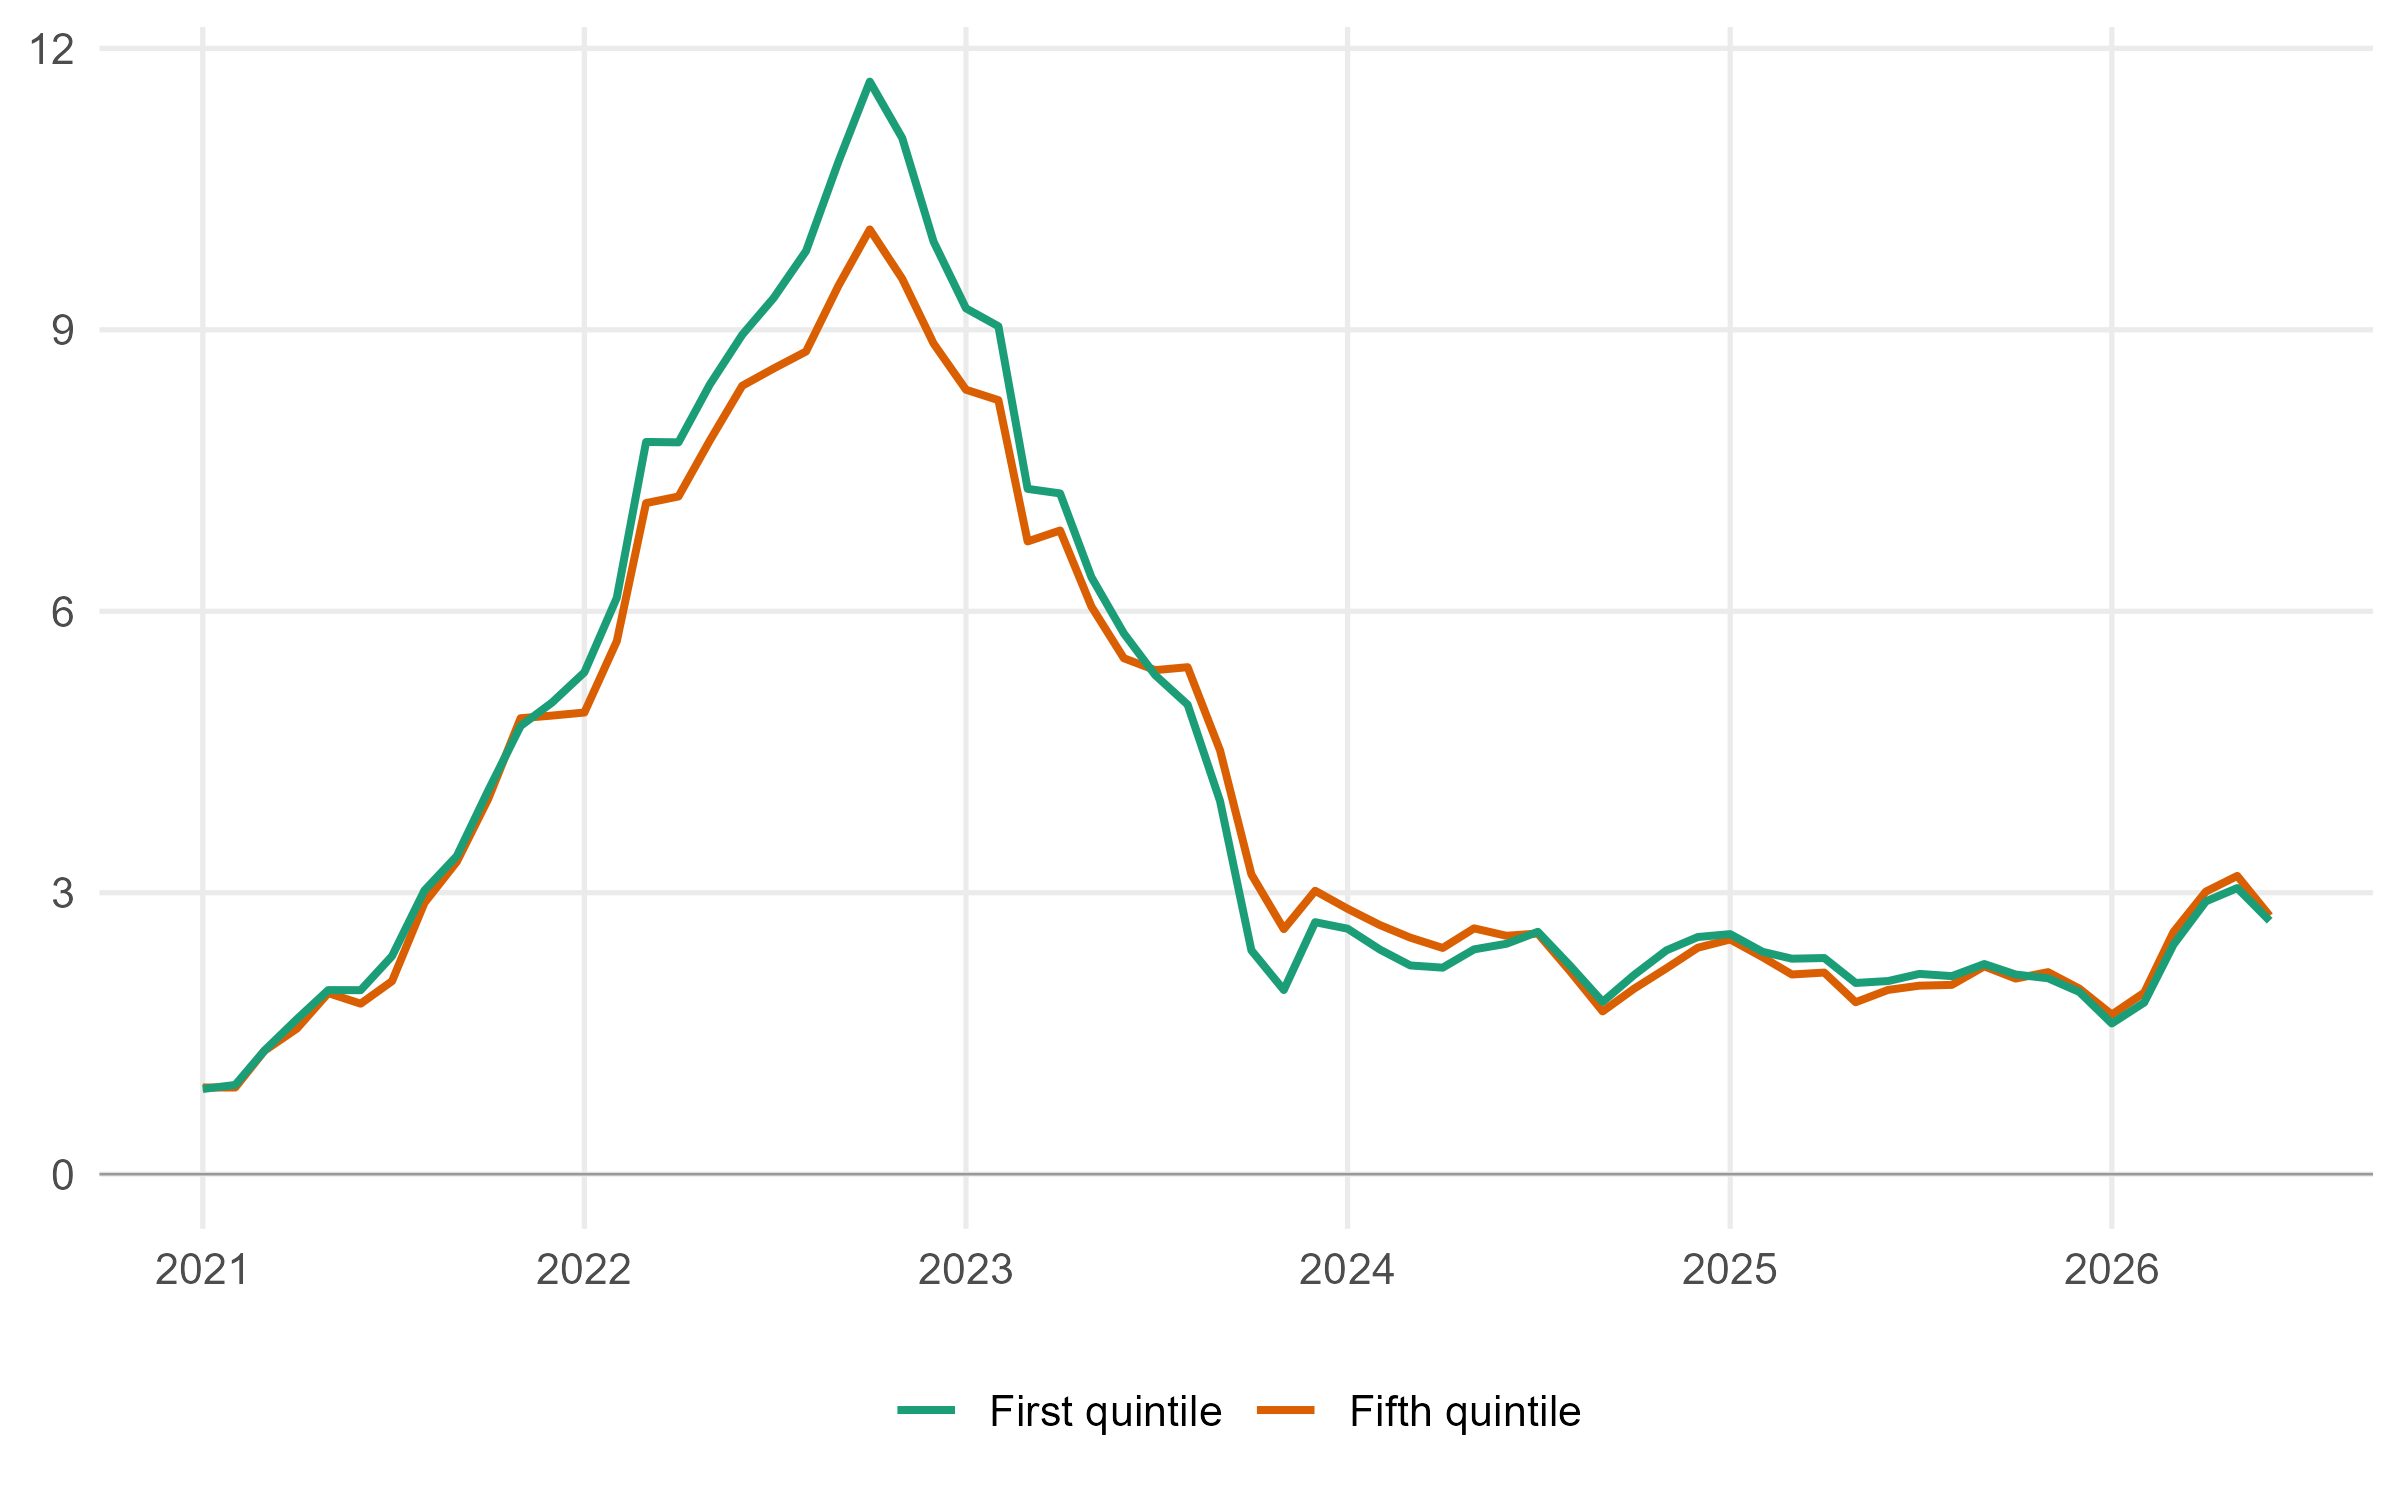
\includegraphics[width=0.82\textwidth,height=0.70\textheight,keepaspectratio]{fig/fig_EA20_2020_2026_income_inflation_Q1_Q5.png}
\source{Eurostat HICP and HBS; authors' calculations. Units: year-on-year inflation, in percent.}
\end{frame}

% 9
\begin{frame}{Since 2000, Only the 2021--23 Shock Had a Sizable Effect on Inflation Inequality}
\centering
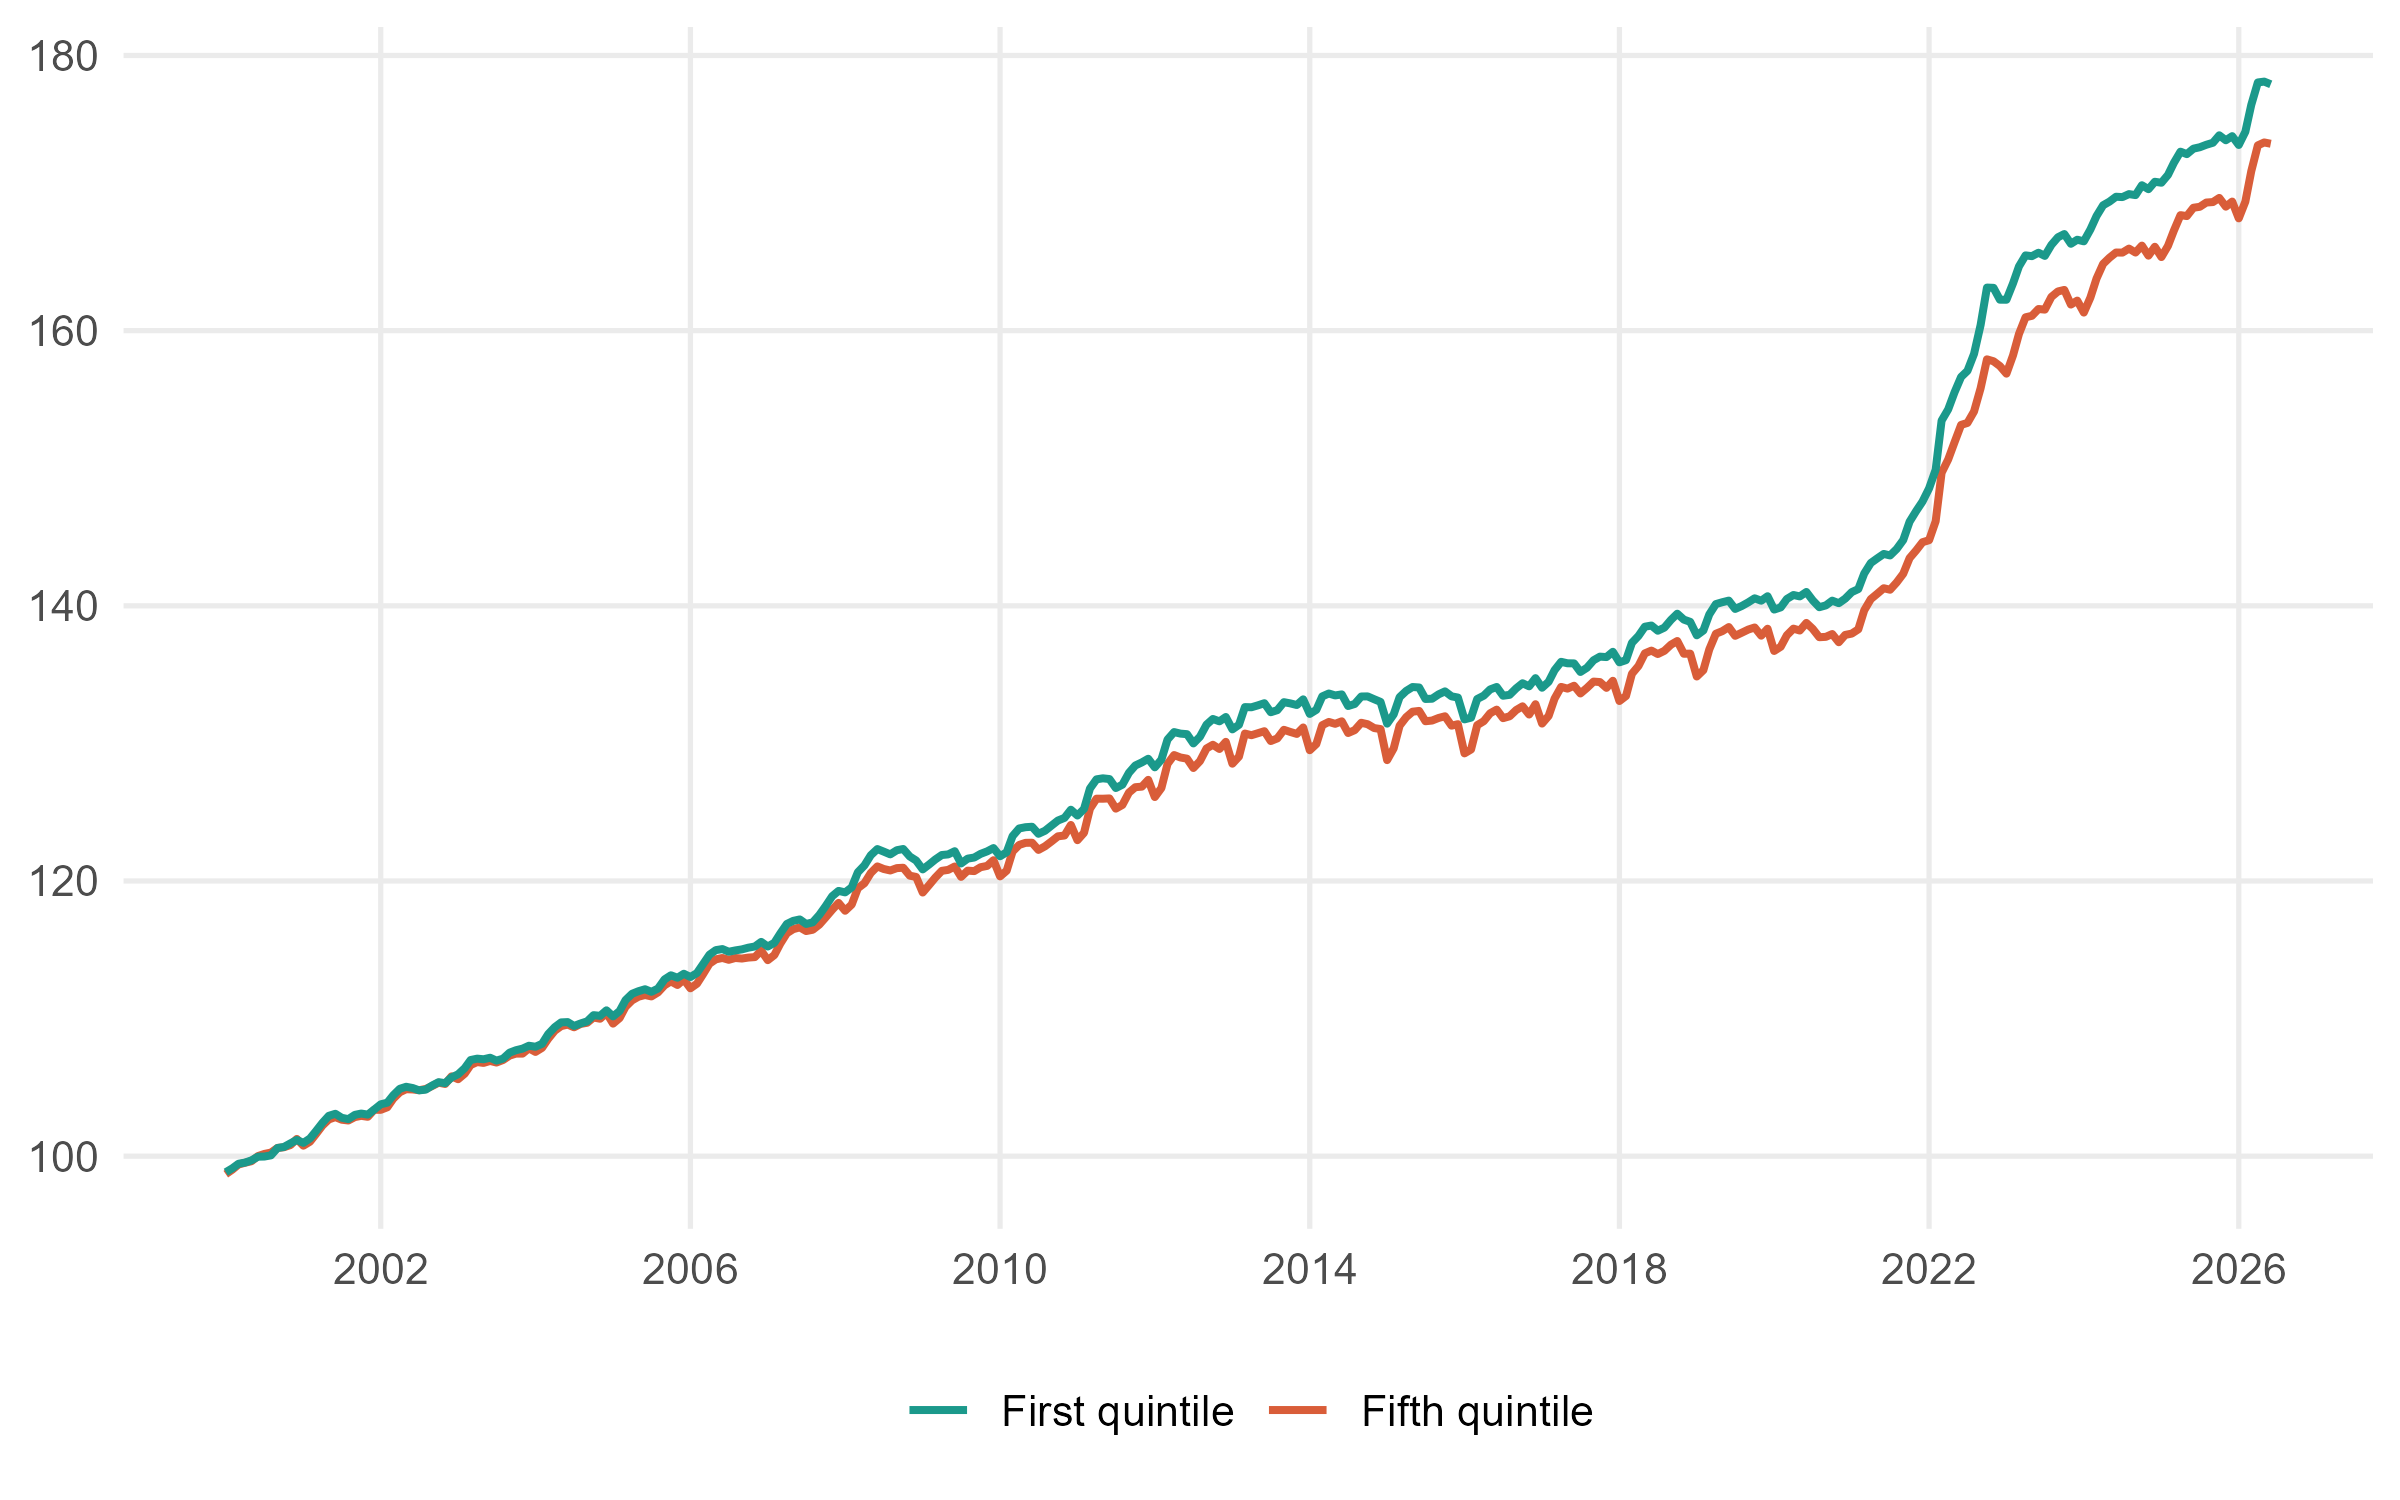
\includegraphics[width=0.82\textwidth,height=0.70\textheight,keepaspectratio]{fig/fig_EA20_2000_2026_income_price_index_Q1_Q5_base2000.png}
\source{Eurostat HICP and HBS; authors' calculations. Units: price index, 2000=100.}
\end{frame}

% 8
\begin{frame}{Heterogeneity in Inflation Gaps Across Countries}
\centering
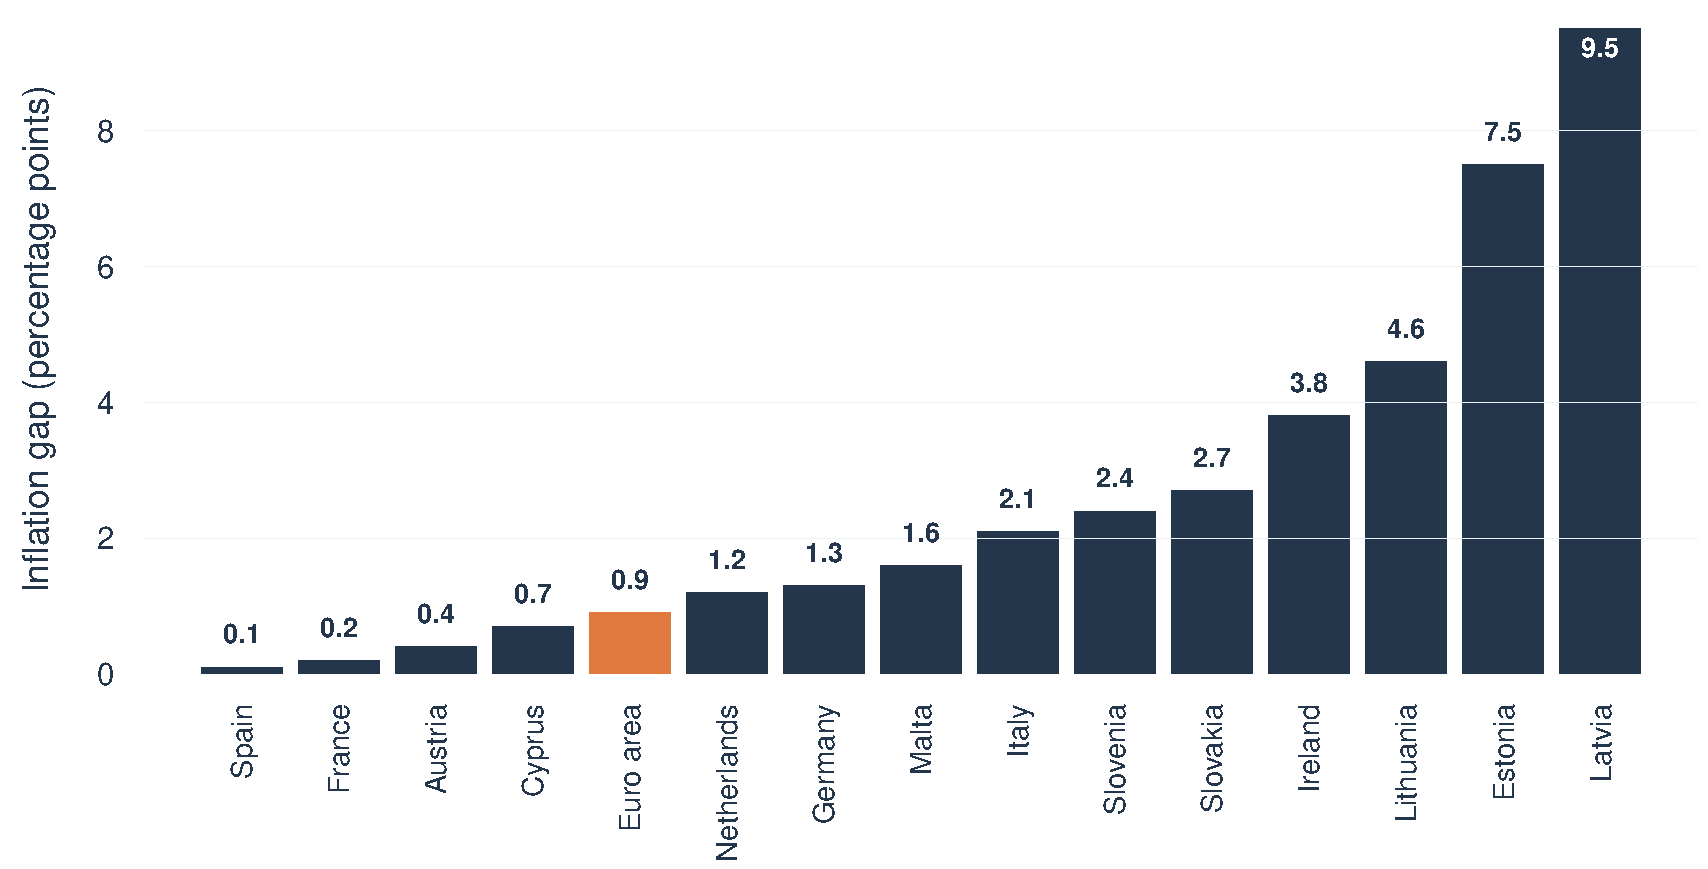
\includegraphics[width=0.99\textwidth,height=0.71\textheight,keepaspectratio]{fig/slide9_country_gaps_excl_pt_fi.pdf}
\source{Eurostat HICP and HBS; authors' calculations. Units: cumulative Q1--Q5 inflation gap, June 2021--June 2023, in percentage points. Portugal and Finland excluded.}
\end{frame}

% 9
\begin{frame}{Energy and Food Widened the Gap; Transport Offset It}
\centering
\small
\begin{tabular}{lrrr>{\columncolor{LightGray}}r}
\toprule
Product group & Headline & Q1 & Q5 & Gap\\
\midrule
Food and non-alcoholic beverages & 4.3 & 5.2 & 4.5 & 0.7\\
Alcohol, tobacco and narcotics & 0.5 & 0.7 & 0.4 & 0.2\\
Clothing and footwear & 0.3 & 0.3 & 0.4 & -0.1\\
Housing, rentals and repairs & 1.2 & 0.4 & 0.6 & -0.2\\
Housing energy & 1.5 & 6.9 & 5.3 & 1.5\\
Transport & 1.9 & 1.6 & 2.8 & -1.2\\
Other & 5.0 & 0.2 & 0.3 & -0.1\\
\midrule
\textbf{Total} & \textbf{14.7} & \textbf{15.2} & \textbf{14.4} & \textbf{0.9}\\
\bottomrule
\end{tabular}
\source{Eurostat HICP and HBS; authors' calculations. Units: contributions to cumulative inflation, June 2021--June 2023, in percentage points.}
\end{frame}


% 5
\begin{frame}{Older Households Faced Higher Inflation}
\centering
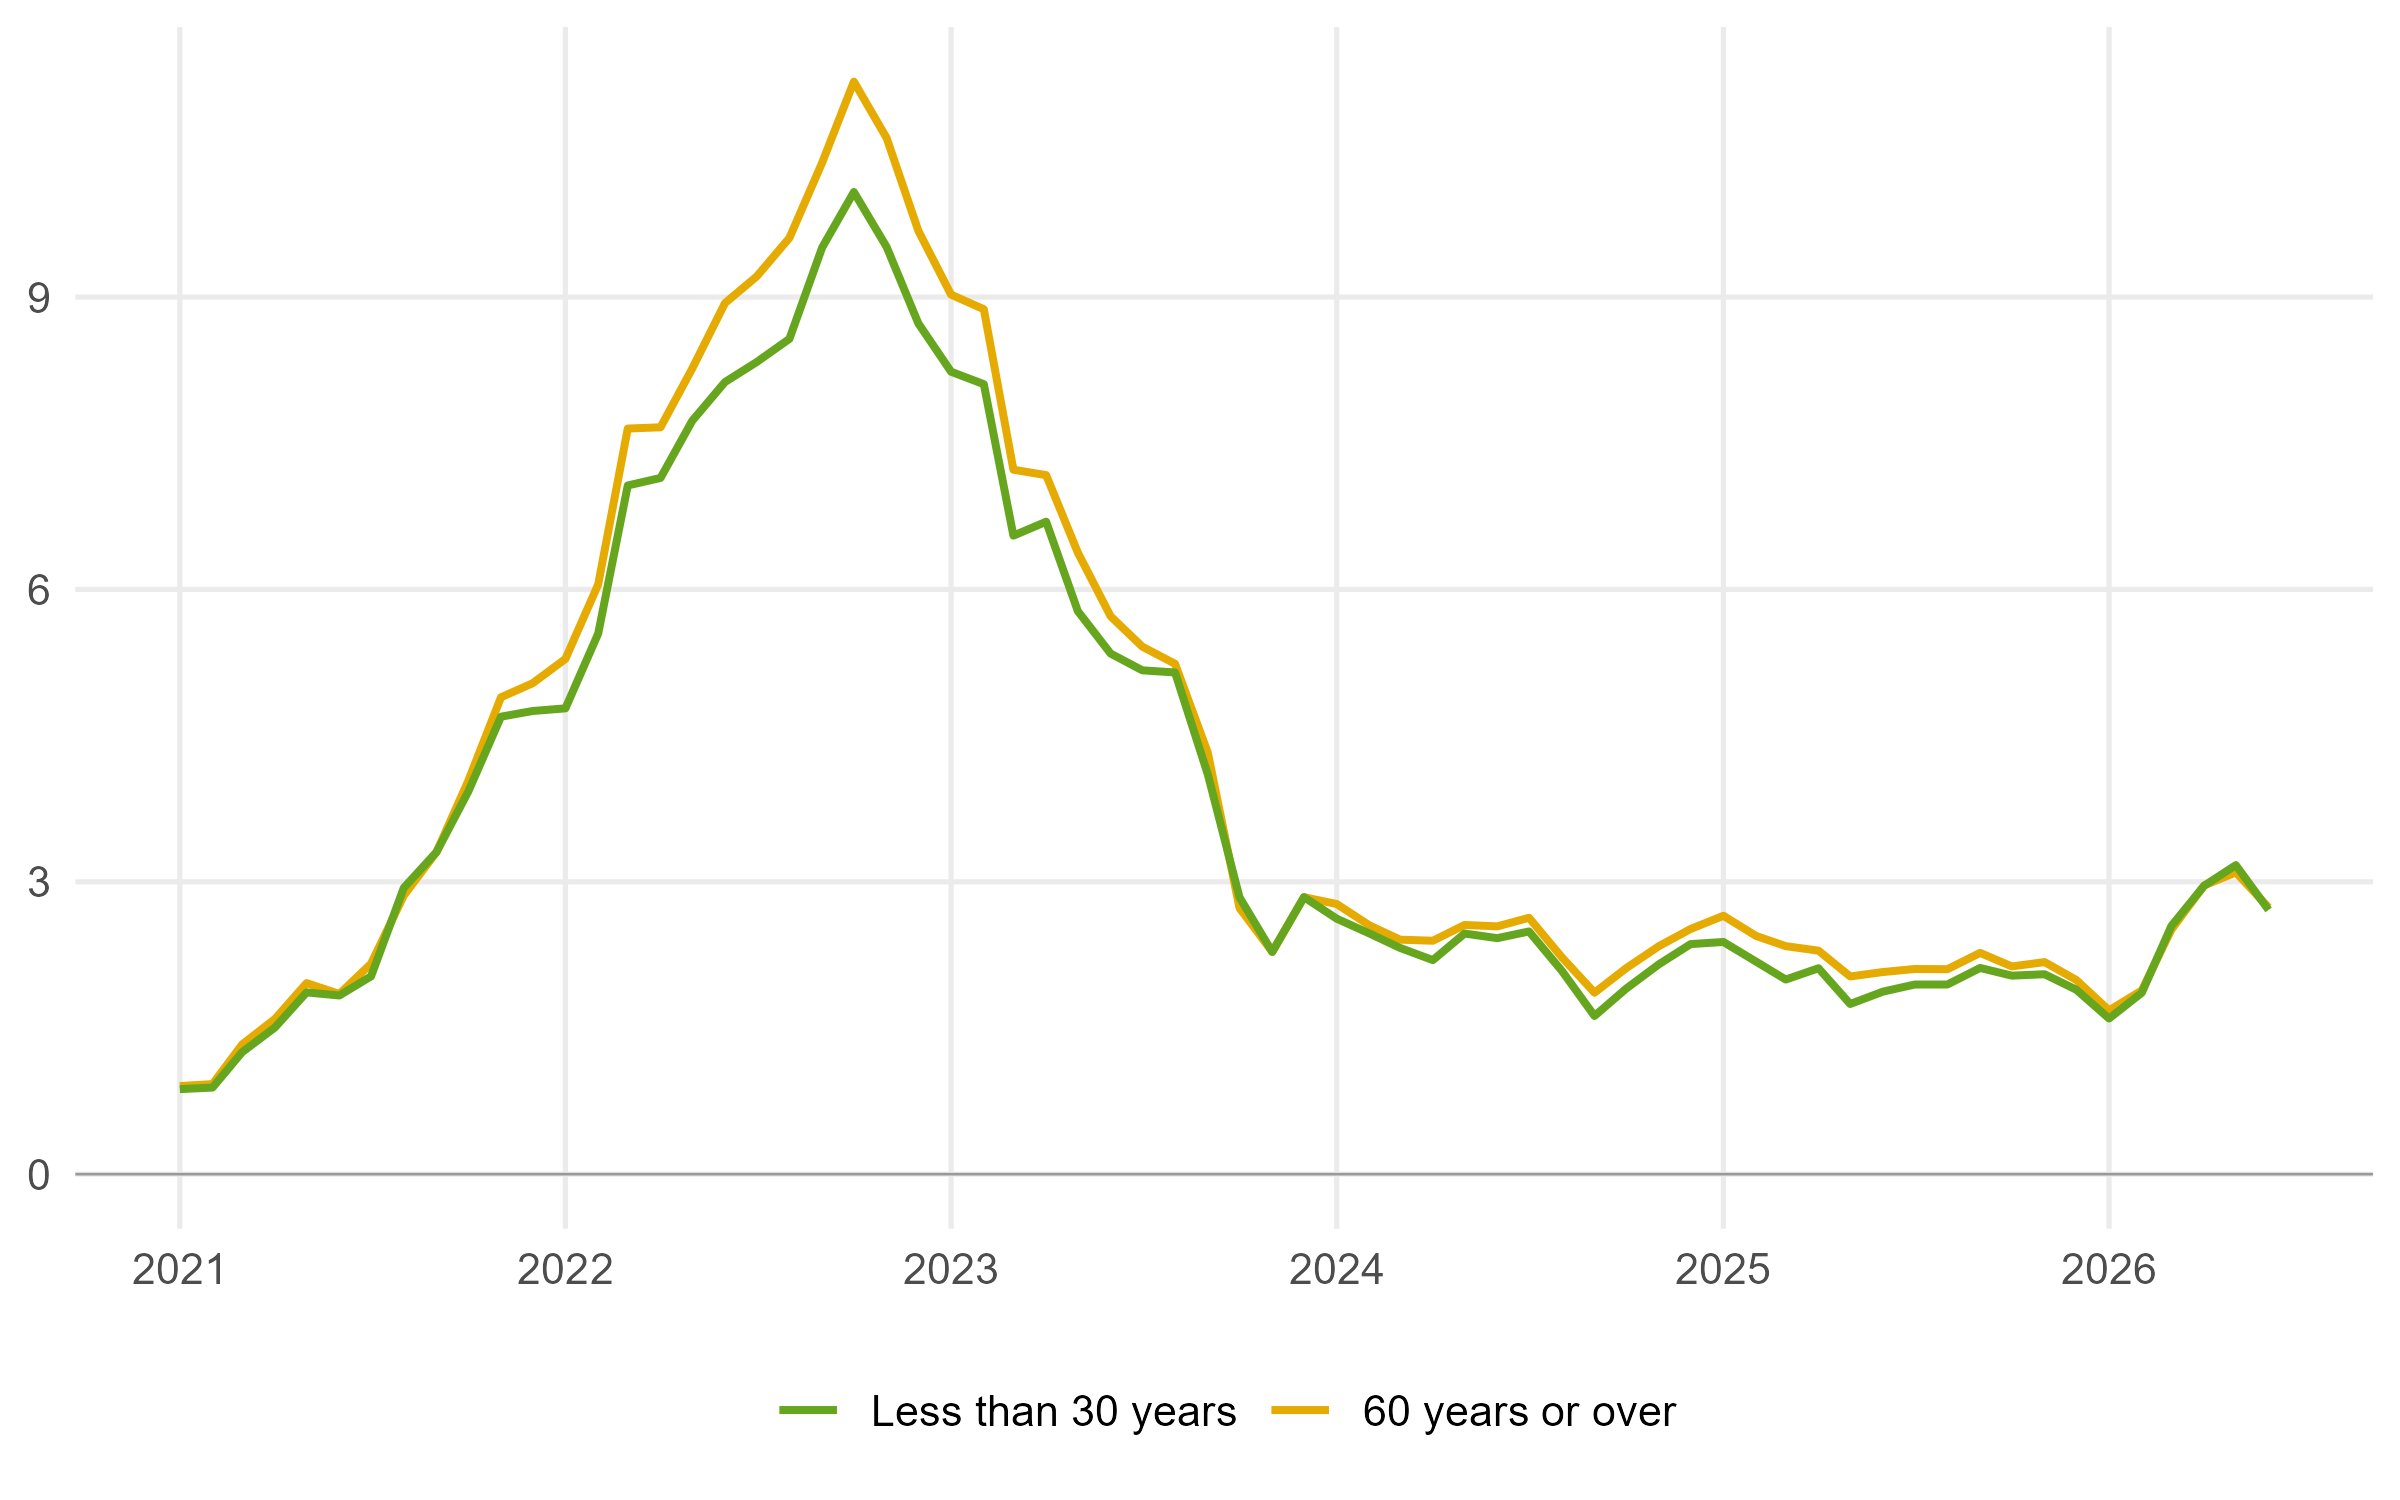
\includegraphics[width=0.82\textwidth,height=0.70\textheight,keepaspectratio]{fig/fig_EA20_2020_2026_age_inflation_under30_60plus.png}
\source{Eurostat HICP and HBS; authors' calculations. Units: year-on-year inflation, in percent.}
\end{frame}

% 8
\begin{frame}{Household-Level Price Indices}
\begin{itemize}
  \item We treat each household as an elementary group. Its individual weight $\omega^{\mathrm{HBS}}_{j,i,2020}$ combines its expenditure on item $j$ with the official HICP weight for that item.
\end{itemize}
\vspace{0.5em}
\[
P_{i,y,m}
=
\sum_{j \in \mathcal{J}_{i,2020,y}}
\omega^{\mathrm{HBS}}_{j,i,2020}
\frac{p_{j,y,m}}{p_{j,y,0}}.
\]
\vspace{0.5em}
\begin{itemize}
  \item Individual indices measure inflation heterogeneity within income, age, and residence categories, which broad group averages conceal.
  \item This within-category dispersion was substantial during the 2021--2023 inflation surge.
\end{itemize}
\end{frame}

% 8 -- formerly slide 24
\begin{frame}{Household Groups Hide Household-Level Dispersion}
\centering
{\small\color{WarmGray}Average inflation and dispersion were both higher in 2022.\par}
\vspace{0.15em}
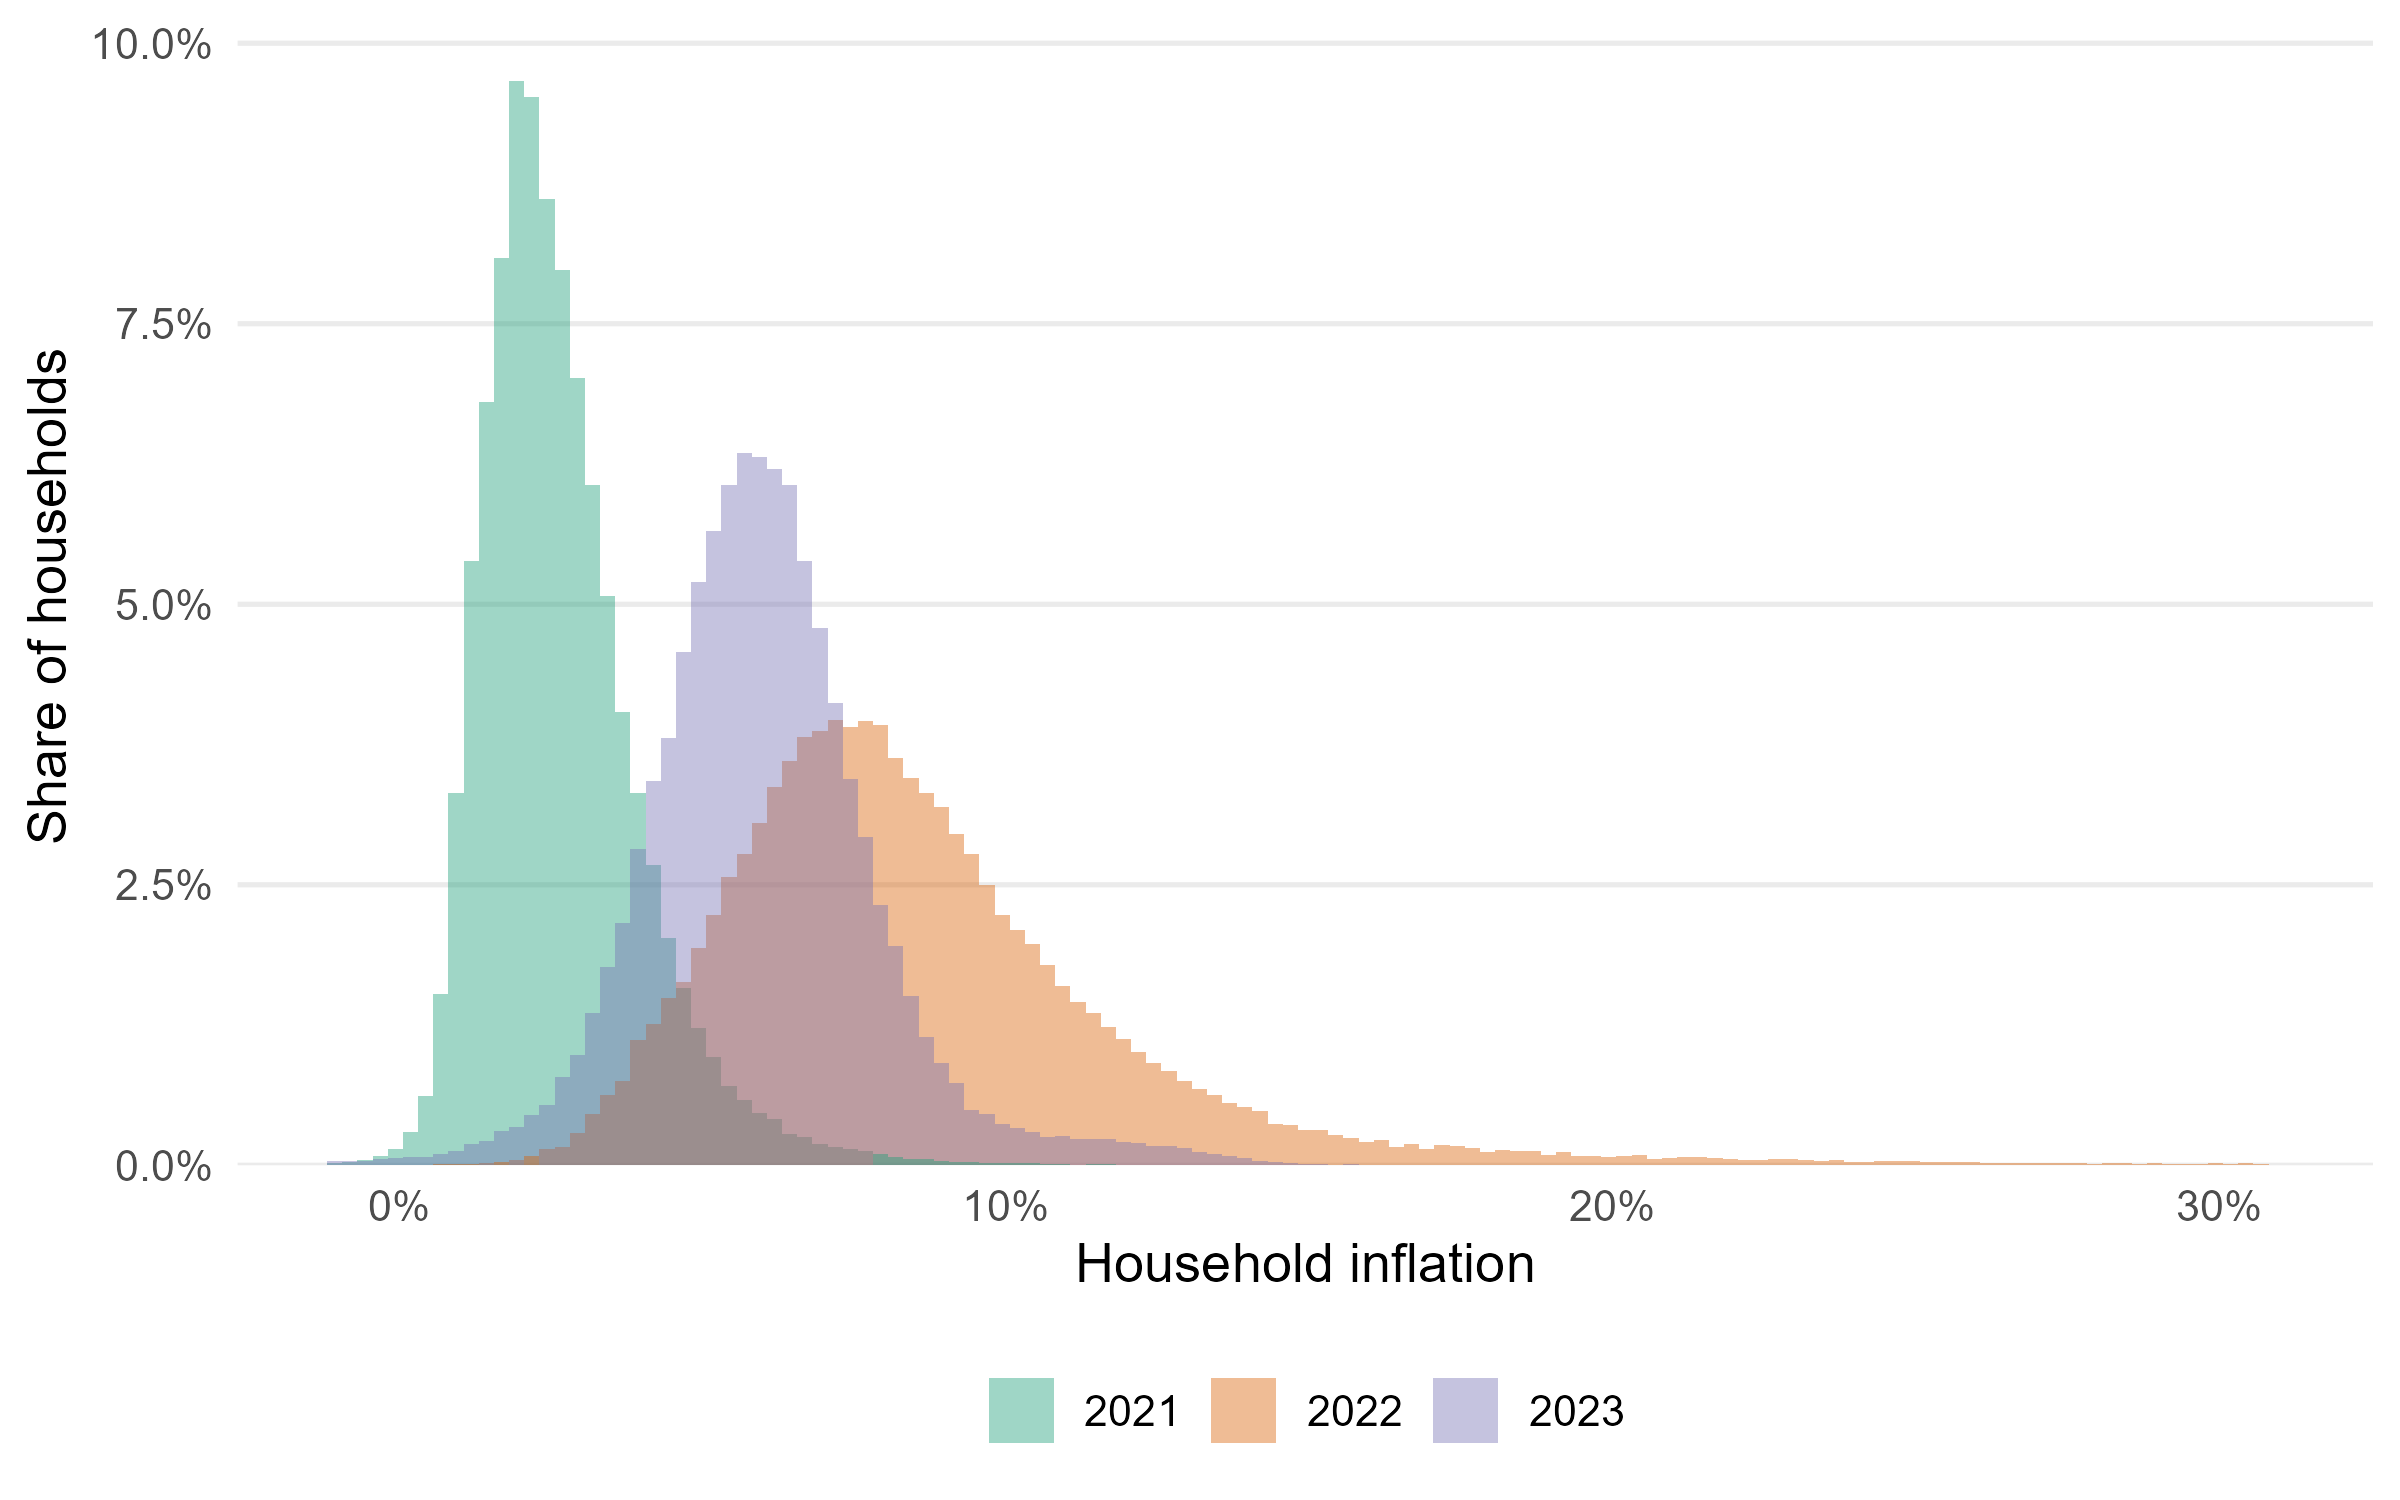
\includegraphics[width=0.96\textwidth,height=0.65\textheight,keepaspectratio]{fig/fig_EA20_household_inflation_distribution_2021_2023.png}
\source{Eurostat HICP and HBS microdata; authors' calculations. Units: annual household inflation (x) and household share (y), in percent.}
\end{frame}


% 11
\begin{frame}{Three Instruments Lowered Retail Energy Prices}
\small
\begin{itemize}
  \item Euro-area price policies cost \textbf{EUR 268 billion}; most were untargeted (\textbf{EUR 235.2 billion, or 88\%}).
  \item \textbf{Price caps and tariff shields} limited household electricity and gas prices.\\
  \textit{Exemple : en France, tarifs réglementés du gaz gelés à leur niveau d'\textbf{octobre 2021} dès novembre 2021 et hausse du tarif réglementé de l'électricité plafonnée à \textbf{4\%} en février 2022.}
  \item \textbf{Temporary VAT and excise-tax reductions} lowered consumer energy prices.\\
  \textit{Exemple : en France, TICFE sur l'électricité ramenée de \textbf{22,5 EUR/MWh} à \textbf{1 EUR/MWh} de février 2022 à janvier 2023.}
  \item \textbf{Fuel rebates and regulated discounts} reduced prices at the pump.\\
  \textit{Exemple : en France, remise de \textbf{18 centimes par litre} d'avril à août 2022, portée à \textbf{30 centimes} de septembre à mi-novembre 2022.}
\end{itemize}
\source{National policy sources; Sgaravatti et al.; authors' calculations.}
\end{frame}

% 12
\begin{frame}{Defining the Price-Policy Counterfactual}
\begin{itemize}
  \item The counterfactual removes these price-based interventions component by component while retaining observed prices for unaffected products.
\end{itemize}
\vspace{0.4em}
\textbf{Example: reversing a temporary VAT cut}
\[
\widetilde p_{j,t}
=
p_{j,t}
\frac{1+\tau^{0}_{j,t}}{1+\tau^{1}_{j,t}},
\qquad
\tau^{1}_{j,t}=\text{policy rate},\quad
\tau^{0}_{j,t}=\text{no-policy rate}.
\]
\centering
\textit{Belgique : une TVA ramenée de \textbf{21\%} à \textbf{6\%} implique}
\[
\widetilde p_{j,t}=p_{j,t}\frac{1.21}{1.06}\simeq 1.142\,p_{j,t}.
\]
{\small
$j=\text{électricité}$ avec $t=$ mars 2022--décembre 2023.
}
\source{National policy sources, Sgaravatti et al.; authors' calculations.}
\end{frame}

% 13
\begin{frame}{Unconventional Fiscal Policies Lowered Inflation by 1.9 pp}
\centering
\begin{tikzpicture}
  \node[inner sep=0] (policyplot) {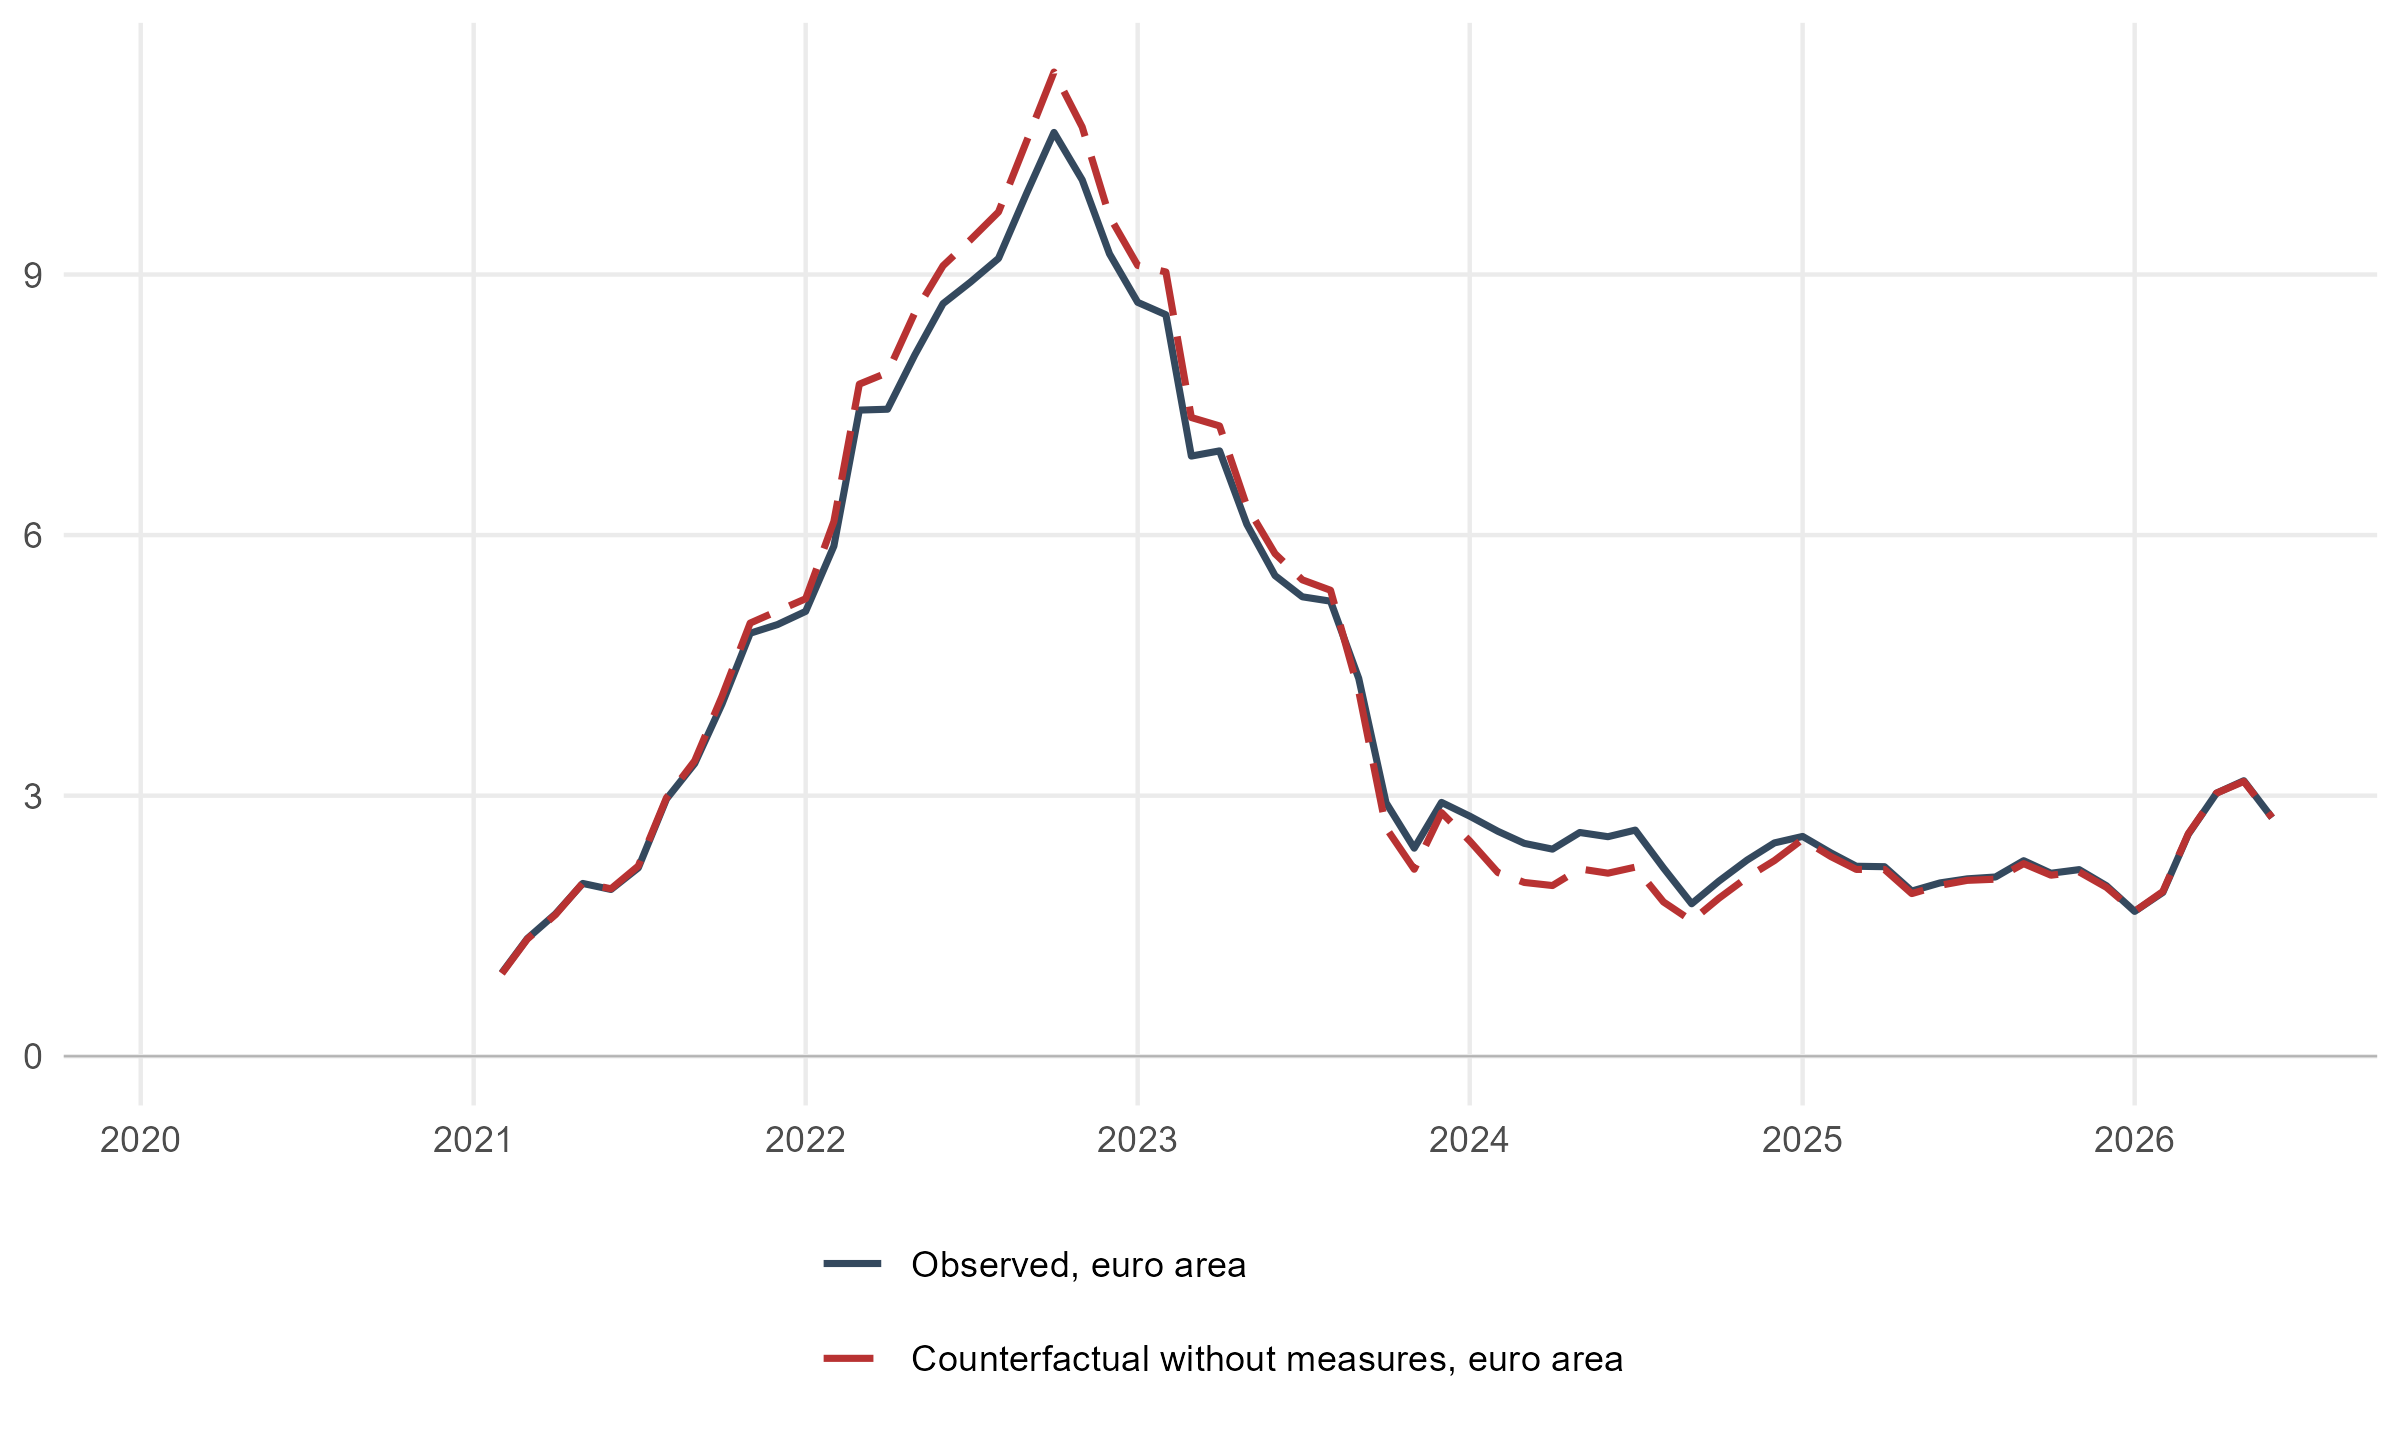
\includegraphics[width=0.86\textwidth,height=0.64\textheight,keepaspectratio,trim=0 70 0 0,clip]{fig/policy_total_cpi_counterfactual_inflation_EA_policy_sample.png}};
  % Plot coordinates aligned with June 2021 and June 2023 on the monthly x-axis.
  \coordinate (policySW) at ($(policyplot.south west)!0.285!(policyplot.south east)$);
  \coordinate (policyNE) at ($(policyplot.north west)!0.558!(policyplot.north east)$);
  \fill[WarmOrange,opacity=0.09] (policySW) rectangle (policyNE);
  \node[anchor=north west,font=\scriptsize\bfseries,text=WarmOrange,
        fill=SoftWhite,fill opacity=0.88,text opacity=1,inner sep=2pt]
        at ($(policyplot.north west)!0.600!(policyplot.north east)+(0,-0.18)$) {Policy period: June 2021--June 2023};
\end{tikzpicture}
\vspace{-0.2em}

{\small\textcolor{DeepNavy}{\rule[0.35ex]{1.3em}{1.1pt}} Observed
\qquad
\textcolor{red!70!black}{\rule[0.35ex]{1.3em}{1.1pt}} No policy}
\source{Eurostat and national statistical institutes; authors' calculations. Units: year-on-year inflation, in percent; January 2021--July 2026.}
\end{frame}

% 12
\begin{frame}{Policies Narrowed the Q1--Q5 Inflation Gap}
\centering
{\small
\[
\Delta\text{Gap}
=
\underbrace{\Delta Q1}_{\text{policy effect}}
-
\underbrace{\Delta Q5}_{\text{policy effect}}
=
\mathbf{-1.1\text{ pp}}
\]
}
\vspace{0.05em}

\begin{columns}[T,onlytextwidth]
  \begin{column}{0.495\textwidth}
    \centering
    {\bfseries Q1}\par\vspace{0.2em}
    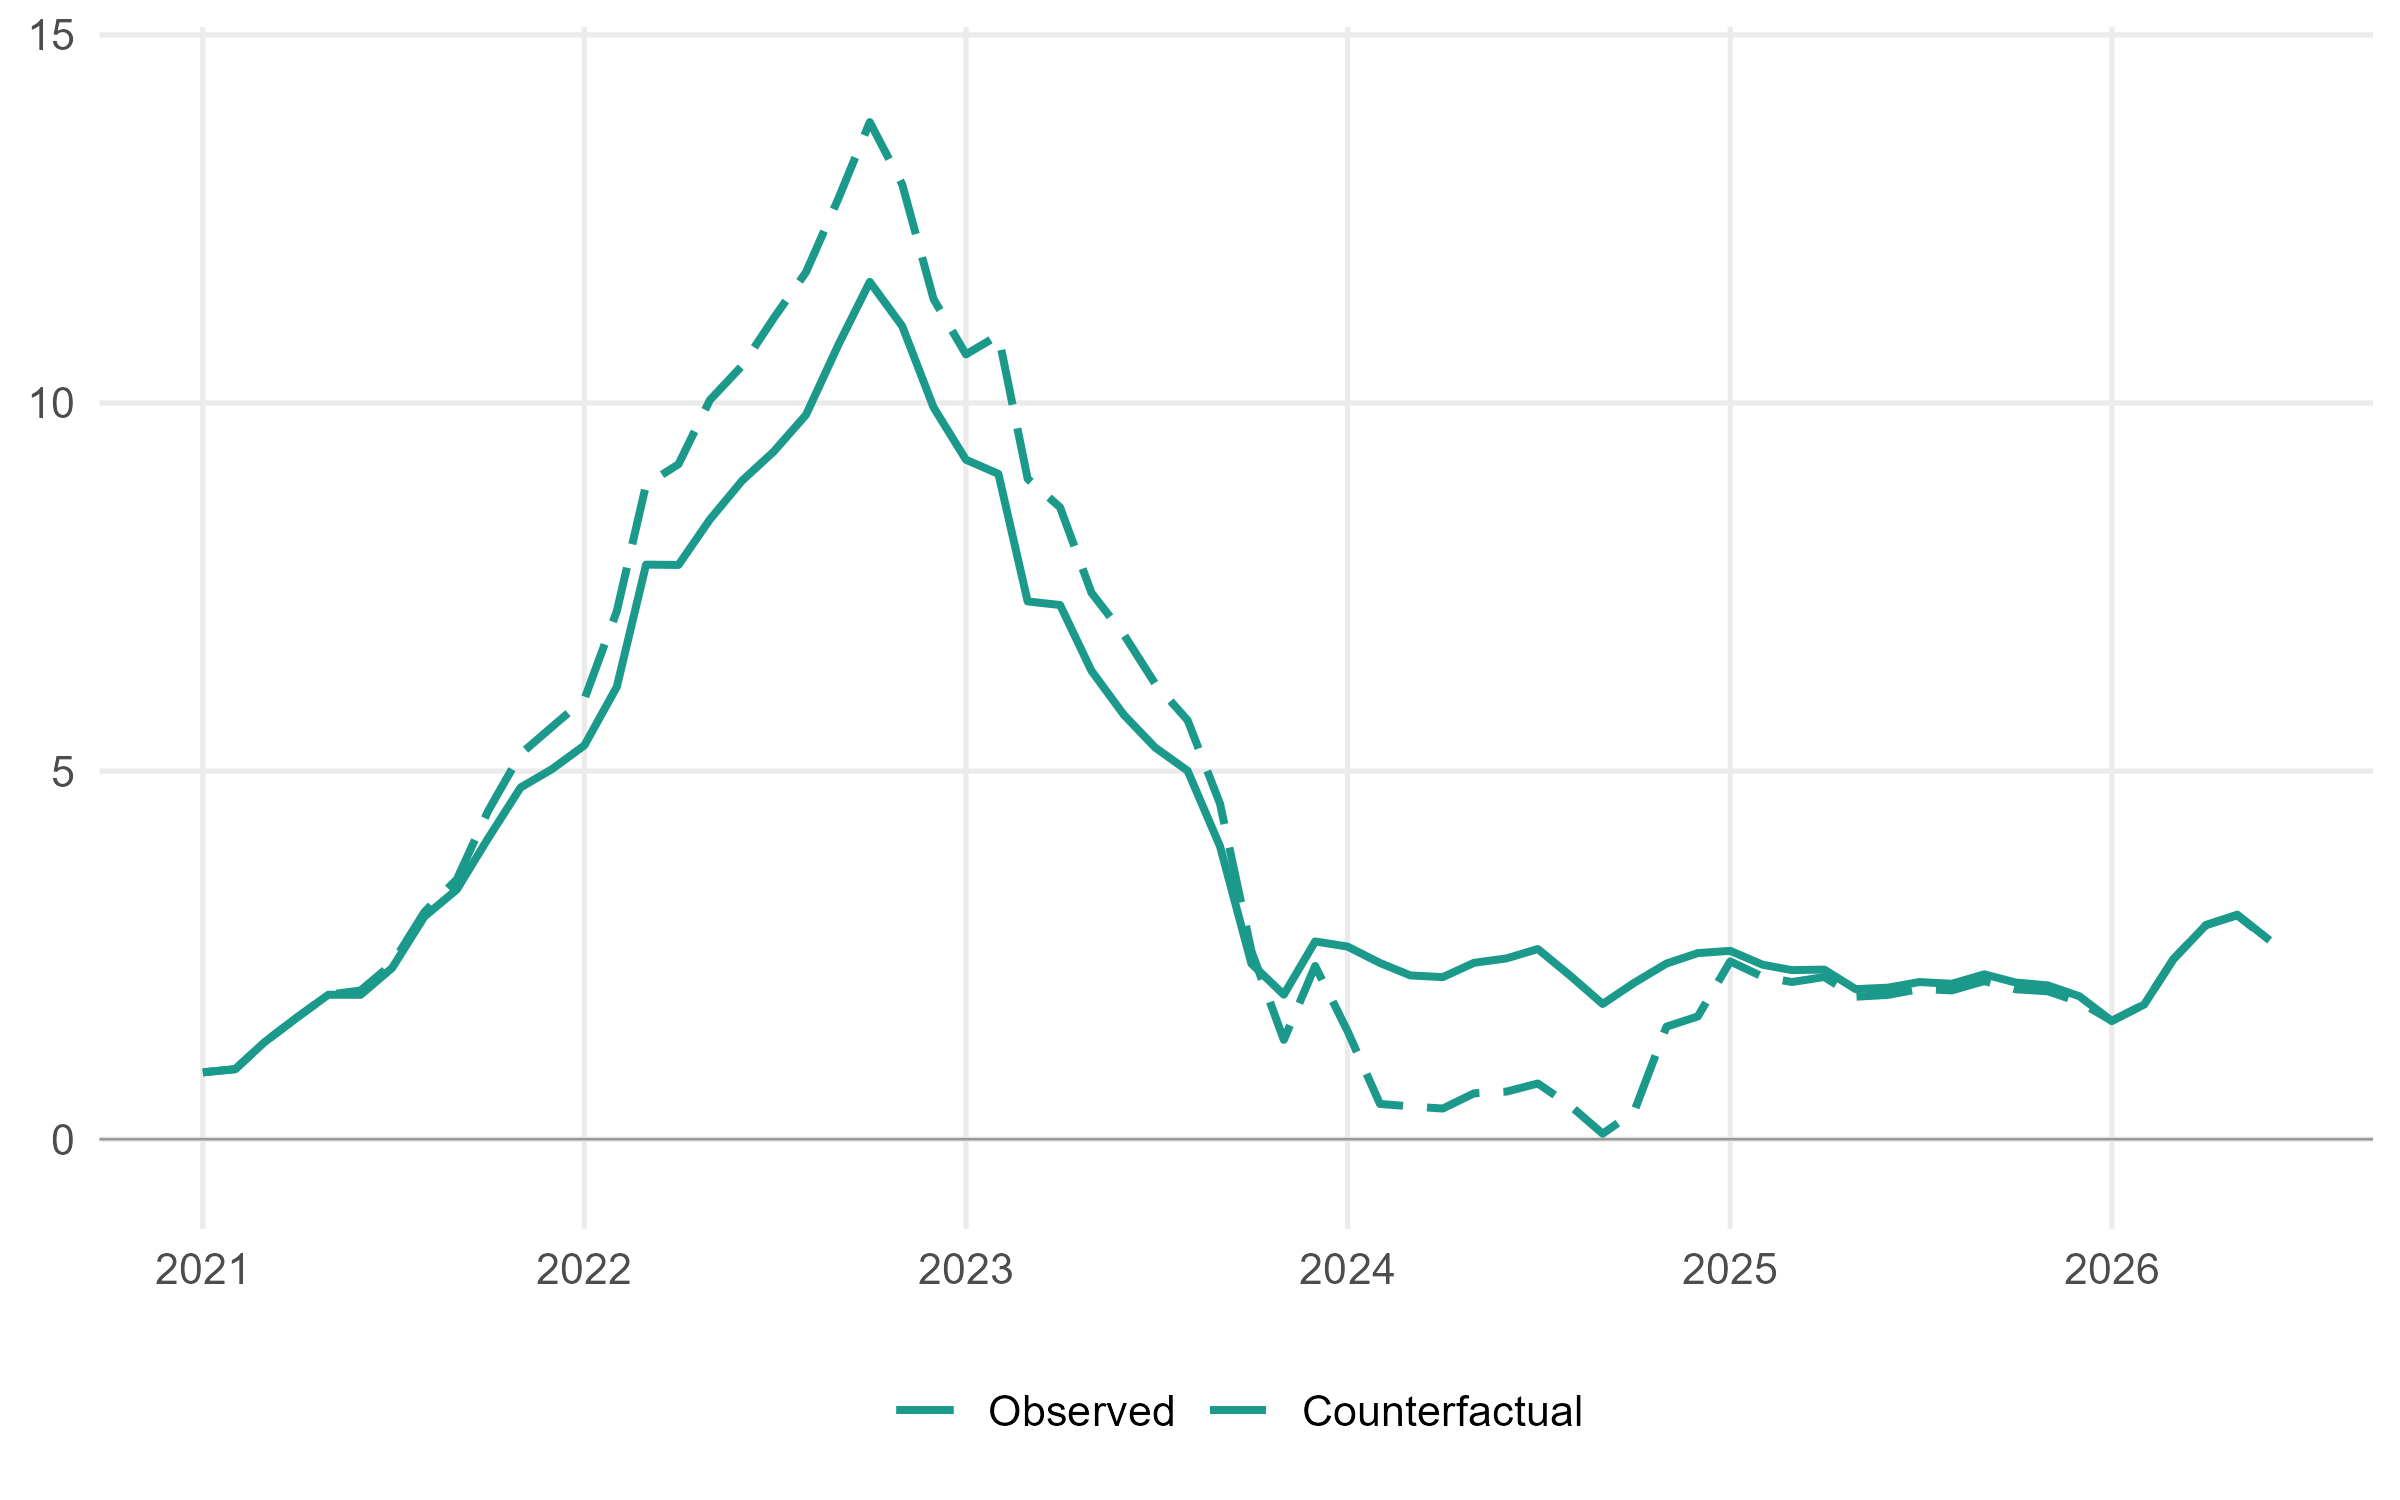
\includegraphics[width=\linewidth,height=0.46\textheight,keepaspectratio]{fig/fig_EA20_2021_2026_counterfactual_income_inflation_Q1.png}
  \end{column}
  \begin{column}{0.495\textwidth}
    \centering
    {\bfseries Q5}\par\vspace{0.2em}
    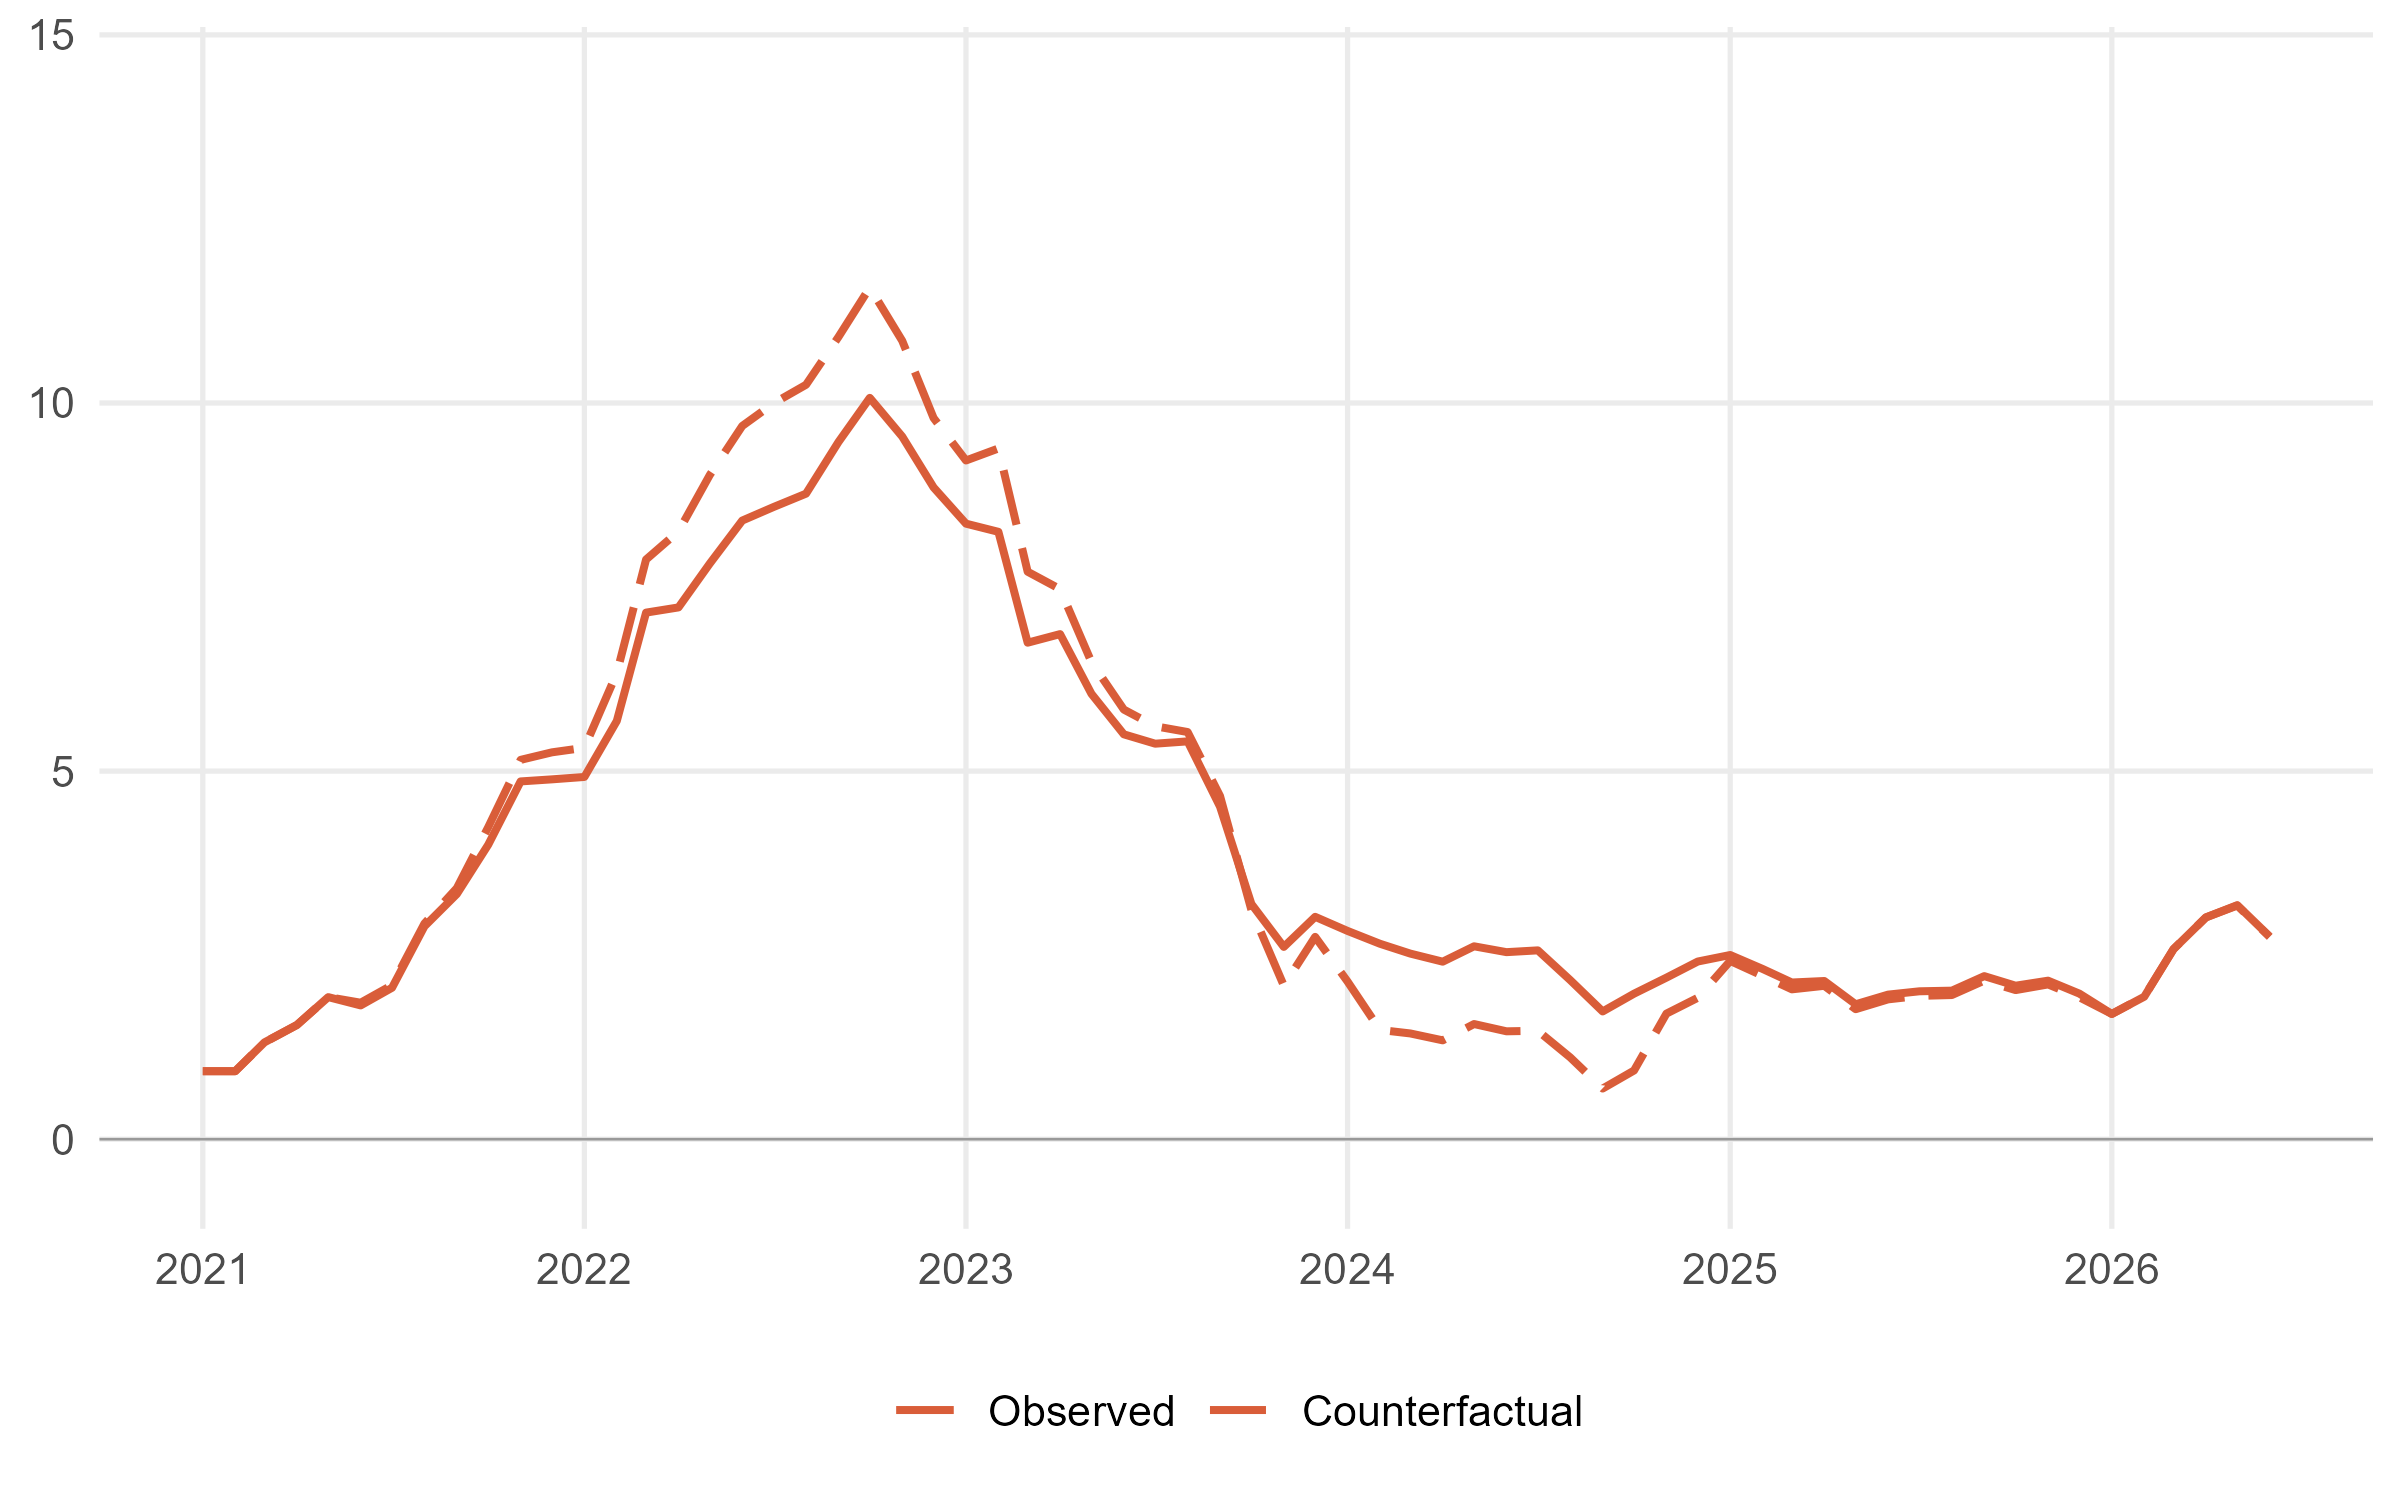
\includegraphics[width=\linewidth,height=0.46\textheight,keepaspectratio]{fig/fig_EA20_2021_2026_counterfactual_income_inflation_Q5.png}
  \end{column}
\end{columns}
\source{Eurostat and national statistical institutes; authors' calculations. Units: year-on-year inflation, in percent; Jan. 2021--July 2026.}
\end{frame}

% 17
\begin{frame}{Conclusion}
\begin{itemize}
  \item The euro-area inflation gap was \textbf{0.9 point}, but cross-country differences were large; age and residence also identify vulnerable households.
  \item Housing energy and food widened the inflation gap, while transport partly offset it; production networks added indirect exposure.
  \item Unconventional fiscal policies lowered cumulative average inflation by \textbf{1.9 points} and the Q1--Q5 gap by \textbf{1.1 points}.
  \item The positive distributional effect came mainly from measures on housing energy, while fuel measures are regressive.
\end{itemize}
\end{frame}

% Appendix begins here; the explicit transition and footline provide the visual marker.
\setbeamertemplate{footline}{%
  \hfill\raisebox{0.6em}{\scriptsize\color{WarmGray}Appendix \insertframenumber/\inserttotalframenumber}\hspace{1em}}

\begin{frame}[plain]
  \centering
  \vfill
  {\Huge\bfseries Appendix\par}
  \vfill
\end{frame}

% A1 -- formerly slide 16
\begin{frame}{Effects of Unconventional Fiscal Policies}
\centering
\scriptsize
\setlength{\tabcolsep}{4pt}
\begin{tabular}{lrrrrr}
\toprule
Country & Fiscal cost & No-policy & Avg. effect & Inflation gap & Effect of fiscal policies\\
 & (EUR bn) & inflation & (pp) & (pp) & (pp)\\
\midrule
Austria & 3.8 & 18.4 & -1.2 & 1.1 & -0.7\\
Estonia & 0.2 & 33.1 & -0.1 & 7.6 & -0.1\\
France & 80.5 & 16.9 & -4.7 & 2.4 & -2.2\\
Germany & 60.2 & 16.5 & -0.8 & 2.2 & -0.9\\
Ireland & 1.4 & 15.0 & -0.1 & 4.0 & -0.2\\
Italy & 36.2 & 16.4 & -0.6 & 2.4 & -0.3\\
Latvia & 0.7 & 28.9 & 0.0 & 10.2 & -0.7\\
Netherlands & 34.8 & 19.5 & -2.6 & 2.2 & -0.9\\
Portugal & 5.9 & 17.0 & -2.9 & -0.8 & -1.5\\
Slovakia & 2.3 & 28.6 & -3.3 & 4.8 & -2.1\\
Spain & 23.9 & 14.3 & -2.5 & 1.3 & -1.2\\
\midrule
\textbf{Euro area} & \textbf{268.0} & \textbf{16.6} & \textbf{-1.9} & \textbf{2.0} & \textbf{-1.1}\\
\bottomrule
\end{tabular}
\vspace{0.5em}
\begin{itemize}
  \item Negative effects indicate that unconventional fiscal policies reduced inflation or the Q1--Q5 gap.
\end{itemize}
\source{Eurostat and national statistical institutes; authors' calculations. Units: fiscal cost in EUR billions; cumulative inflation in percent and policy effects in percentage points, June 2021--June 2023.}
\end{frame}

% A1
\begin{frame}{Rural Households Faced Higher Inflation at the Peak}
\centering
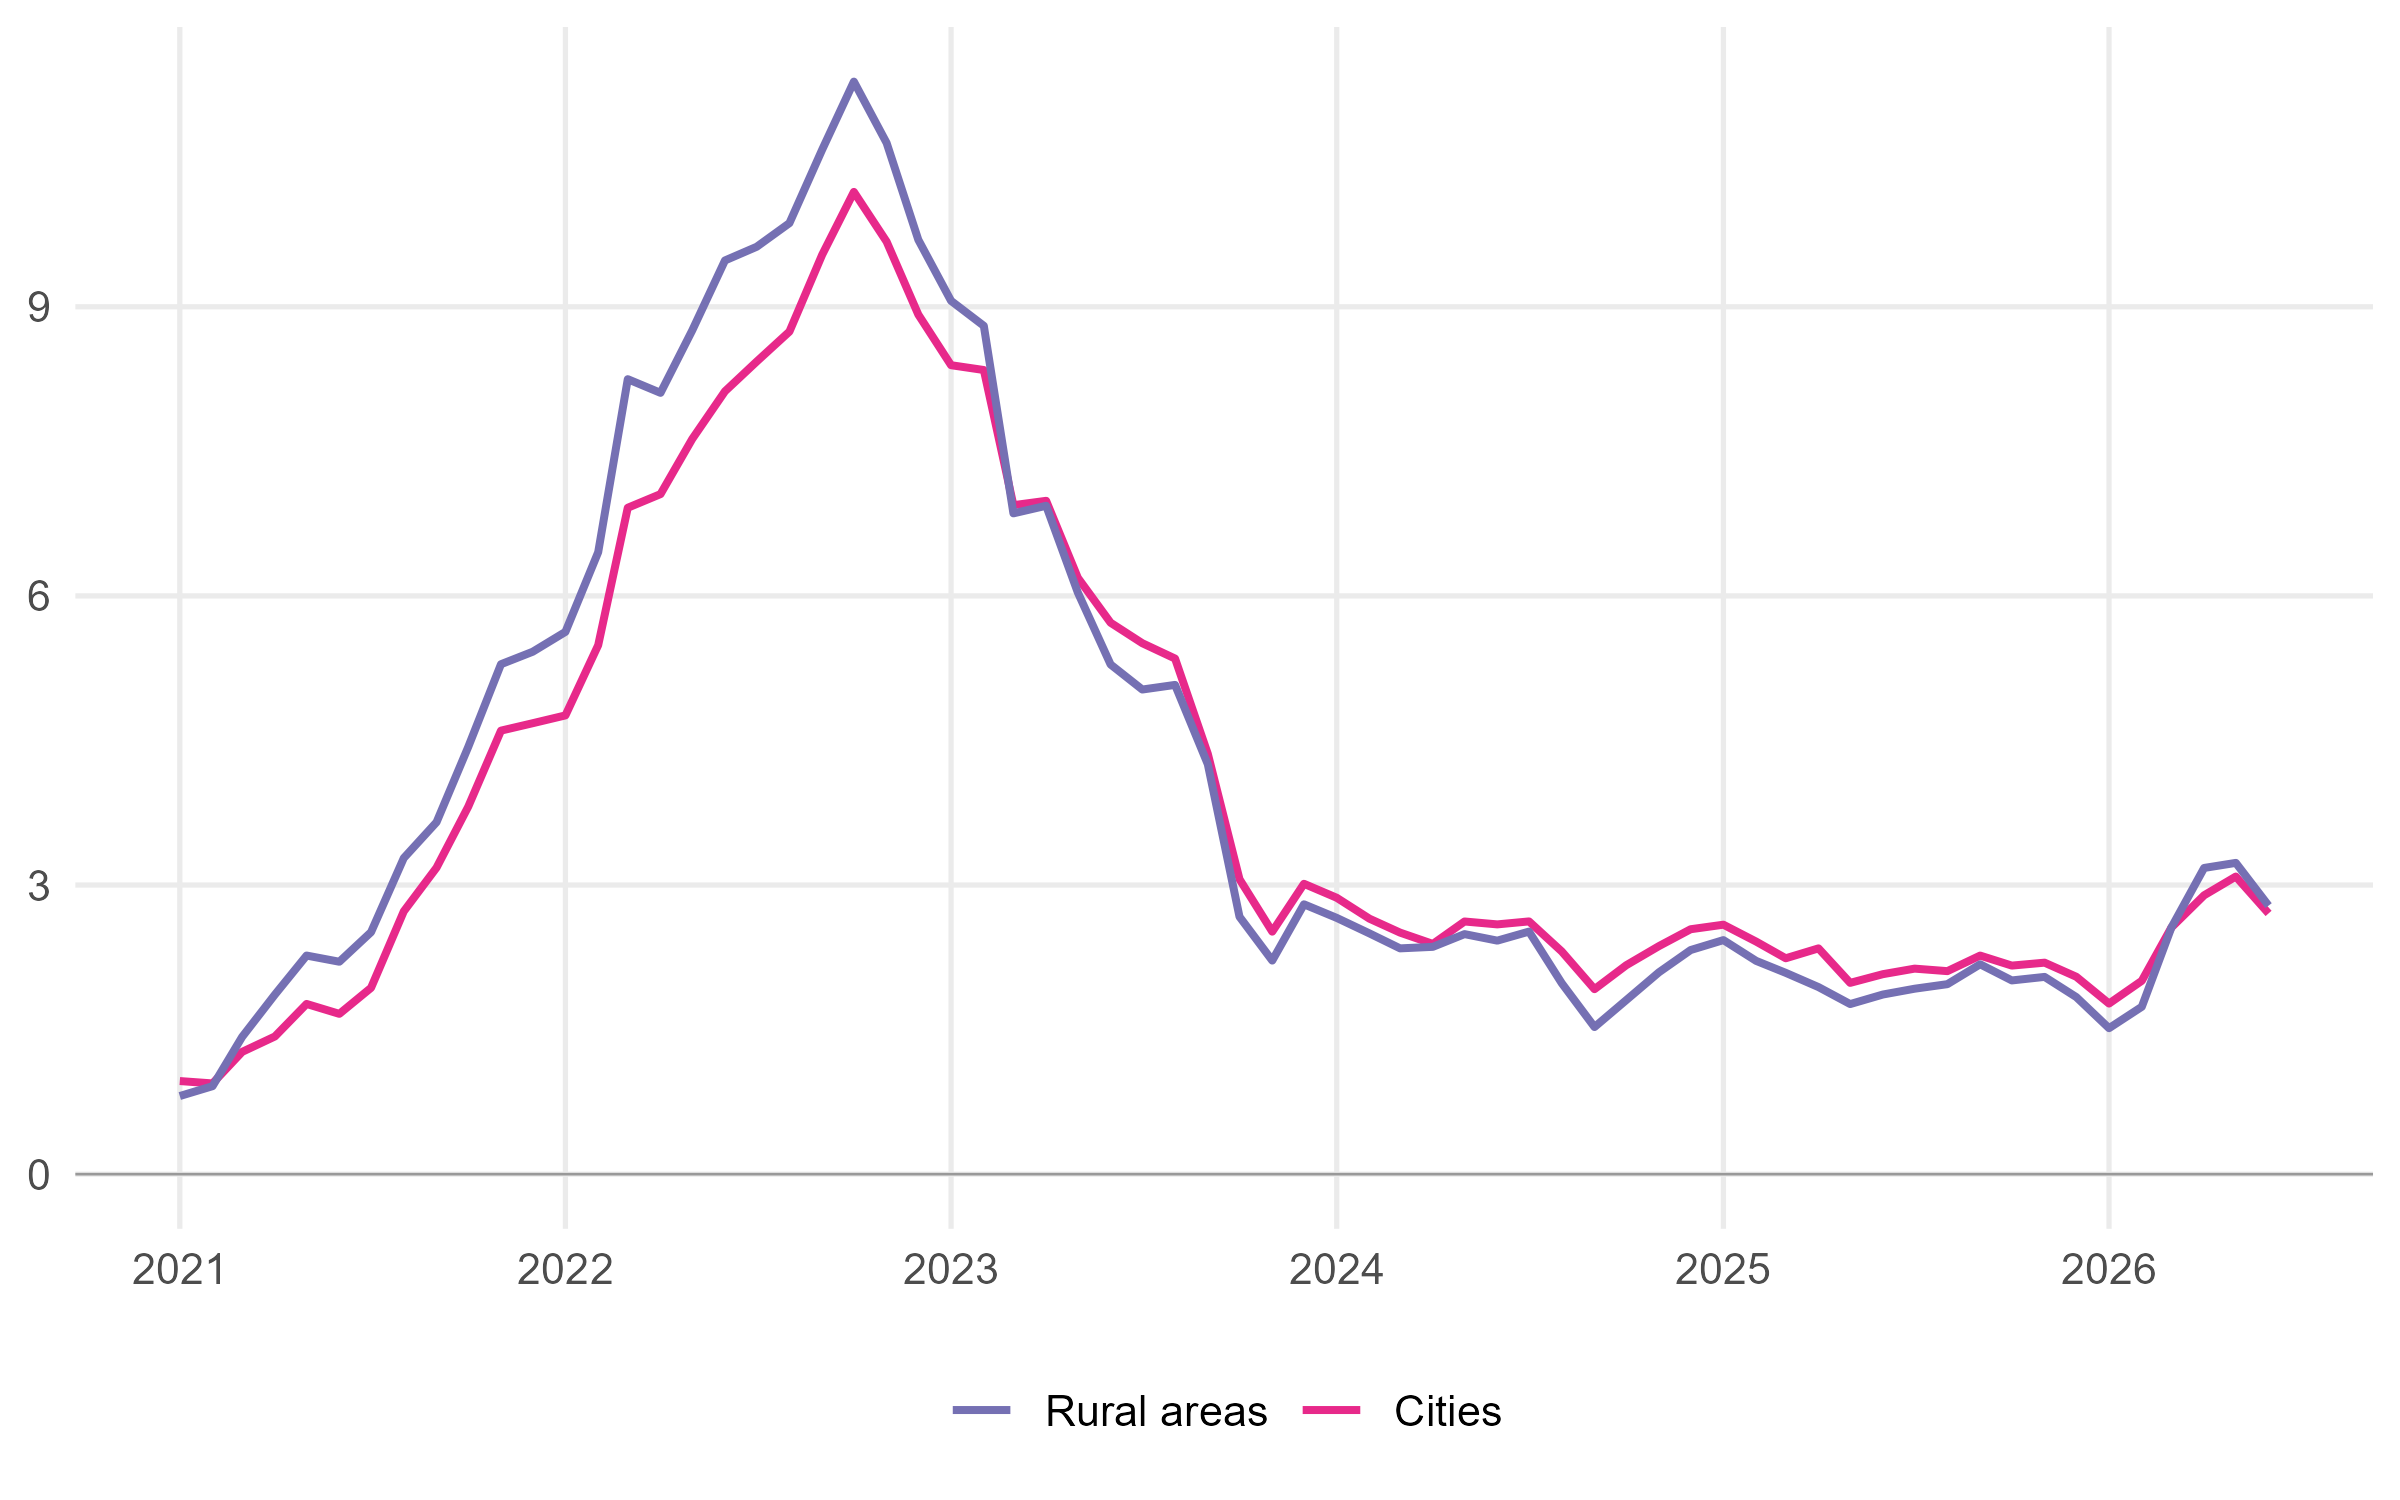
\includegraphics[width=0.78\textwidth,height=0.62\textheight,keepaspectratio]{fig/fig_EA20_2020_2026_urban_inflation_rural_cities.png}
\source{Eurostat HICP and HBS; authors' calculations. Units: year-on-year inflation, in percent.}
\end{frame}

% A2
\begin{frame}{Direct Exposure Explains Most of the Energy-Shock Gap}
\centering
\scriptsize
\begin{tabular}{lrrrrrr}
\toprule
Country & Total & Direct & Indirect & Gap & Gap direct & Gap indirect\\
\midrule
Austria & 3.3 & 1.9 & 1.4 & 0.7 & 0.5 & 0.2\\
Belgium & 4.6 & 2.6 & 1.9 & 1.9 & 1.7 & 0.2\\
Germany & 4.1 & 3.0 & 1.1 & 1.5 & 1.4 & 0.1\\
Estonia & 4.4 & 2.1 & 2.3 & 2.2 & 0.8 & 1.4\\
Spain & 3.1 & 2.2 & 0.9 & 0.2 & 0.1 & 0.1\\
France & 3.2 & 2.3 & 0.8 & 0.6 & 0.6 & 0.0\\
Italy & 5.1 & 3.4 & 1.7 & -0.5 & -0.4 & -0.1\\
Latvia & 4.3 & 3.1 & 1.2 & 3.3 & 2.3 & 1.0\\
Netherlands & 3.7 & 2.9 & 0.8 & 1.4 & 1.4 & 0.0\\
Portugal & 3.0 & 2.0 & 1.1 & 1.1 & 0.9 & 0.2\\
Slovakia & 2.4 & 1.7 & 0.7 & 0.5 & 0.5 & 0.0\\
\midrule
\textbf{Euro area} & \textbf{3.9} & \textbf{2.7} & \textbf{1.1} & \textbf{0.8} & \textbf{0.7} & \textbf{0.1}\\
\bottomrule
\end{tabular}
\vspace{0.5em}
\begin{itemize}
  \item A uniform \textbf{40\%} energy-price shock raises the euro-area Q1--Q5 gap by \textbf{0.8 point}; direct exposure accounts for \textbf{0.7 point}.
\end{itemize}
\source{Eurostat HICP, HBS and FIGARO; authors' calculations. Units: simulated cumulative inflation effects, June 2021--June 2023, in percentage points.}
\end{frame}

% A3 -- formerly slide 15
\begin{frame}{Energy Price Measures Account for the Gap Reduction}
\centering
\small
\begin{tabular}{lrrrrr}
\toprule
Product group & No-policy & Q1 & Q5 & Gap & Policy effect\\
\midrule
Food and non-alcoholic beverages & 4.6 & 5.1 & 4.4 & 0.7 & 0.0\\
Alcohol, tobacco and narcotics & 0.5 & 0.6 & 0.4 & 0.2 & 0.0\\
Clothing and footwear & 0.3 & 0.3 & 0.4 & -0.2 & 0.0\\
Housing, rentals and repairs & 0.5 & 0.4 & 0.6 & -0.2 & 0.0\\
Water, electricity, gas and fuels & 7.8 & 9.7 & 6.8 & 2.9 & -1.4\\
Transport & 2.5 & 1.7 & 3.1 & -1.4 & 0.2\\
Other & 0.3 & 0.2 & 0.4 & -0.1 & 0.0\\
\midrule
\textbf{Total} & \textbf{16.6} & \textbf{18.0} & \textbf{16.1} & \textbf{2.0} & \textbf{-1.1}\\
\bottomrule
\end{tabular}
\vspace{0.7em}
\begin{itemize}
  \item Lower gas and electricity prices reduced the gap by \textbf{1.4 points}; fuel measures increased it by \textbf{0.2 point}.
\end{itemize}
\source{Eurostat and national statistical institutes; authors' calculations. Units: product contributions to cumulative inflation and policy effects, June 2021--June 2023, in percentage points.}
\end{frame}

% A2 -- formerly slide 16
\begin{frame}{RAS-Calibrated Inflation Tracks the Published HICP}
\centering
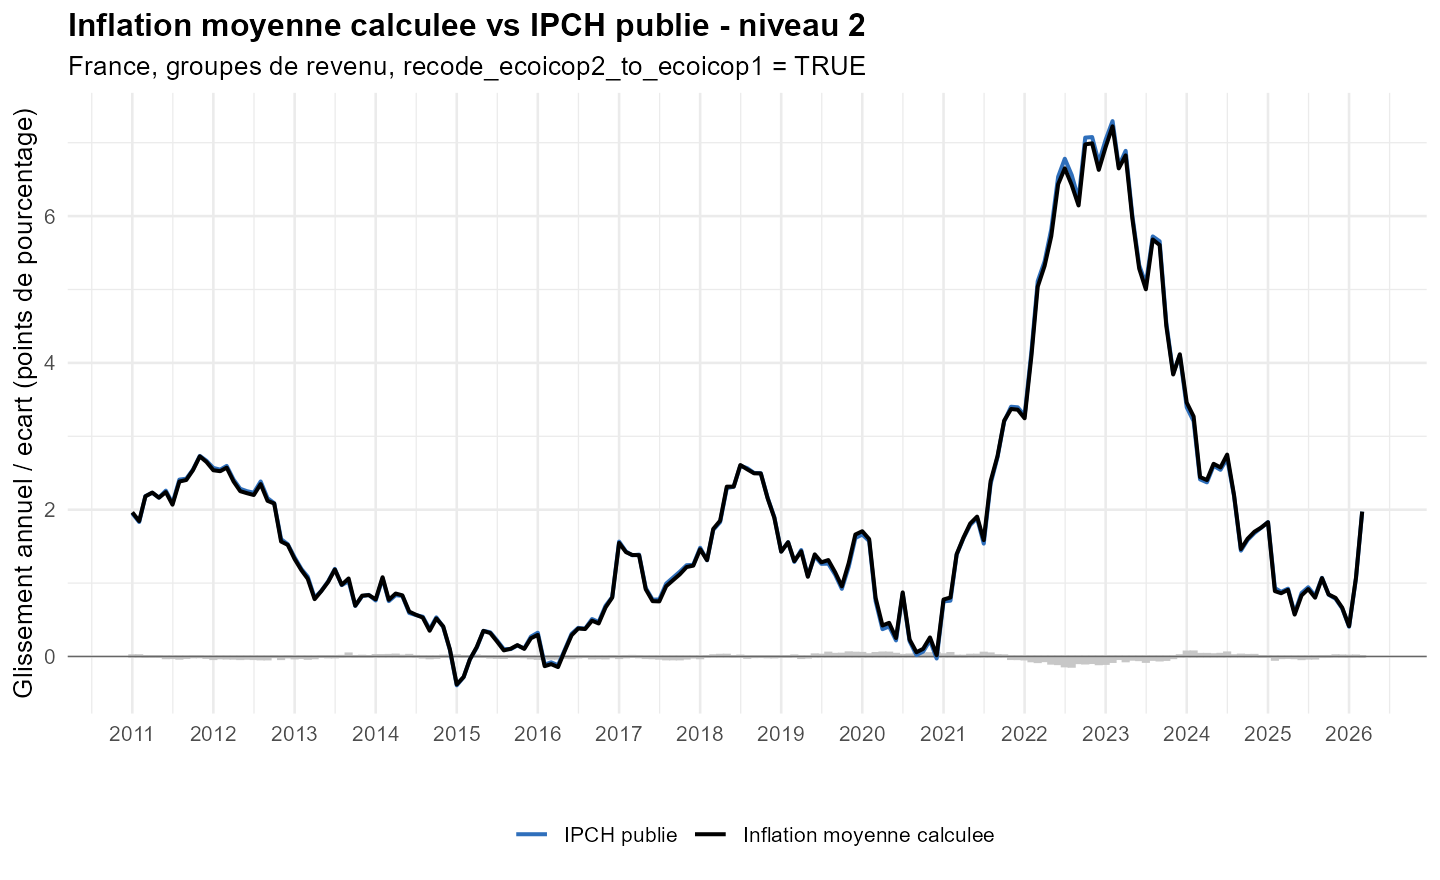
\includegraphics[width=0.96\textwidth,height=0.72\textheight,keepaspectratio]{fig/fig_FR_2010_2026_hicp_inflation_validation_level2_recode_mean_vs_published.png}
\source{INSEE, Eurostat; authors' calculations. Units: year-on-year inflation, in percent.}
\end{frame}

% A3
\begin{frame}{Inflation Burden Is Larger for Low-Income Households}
\centering
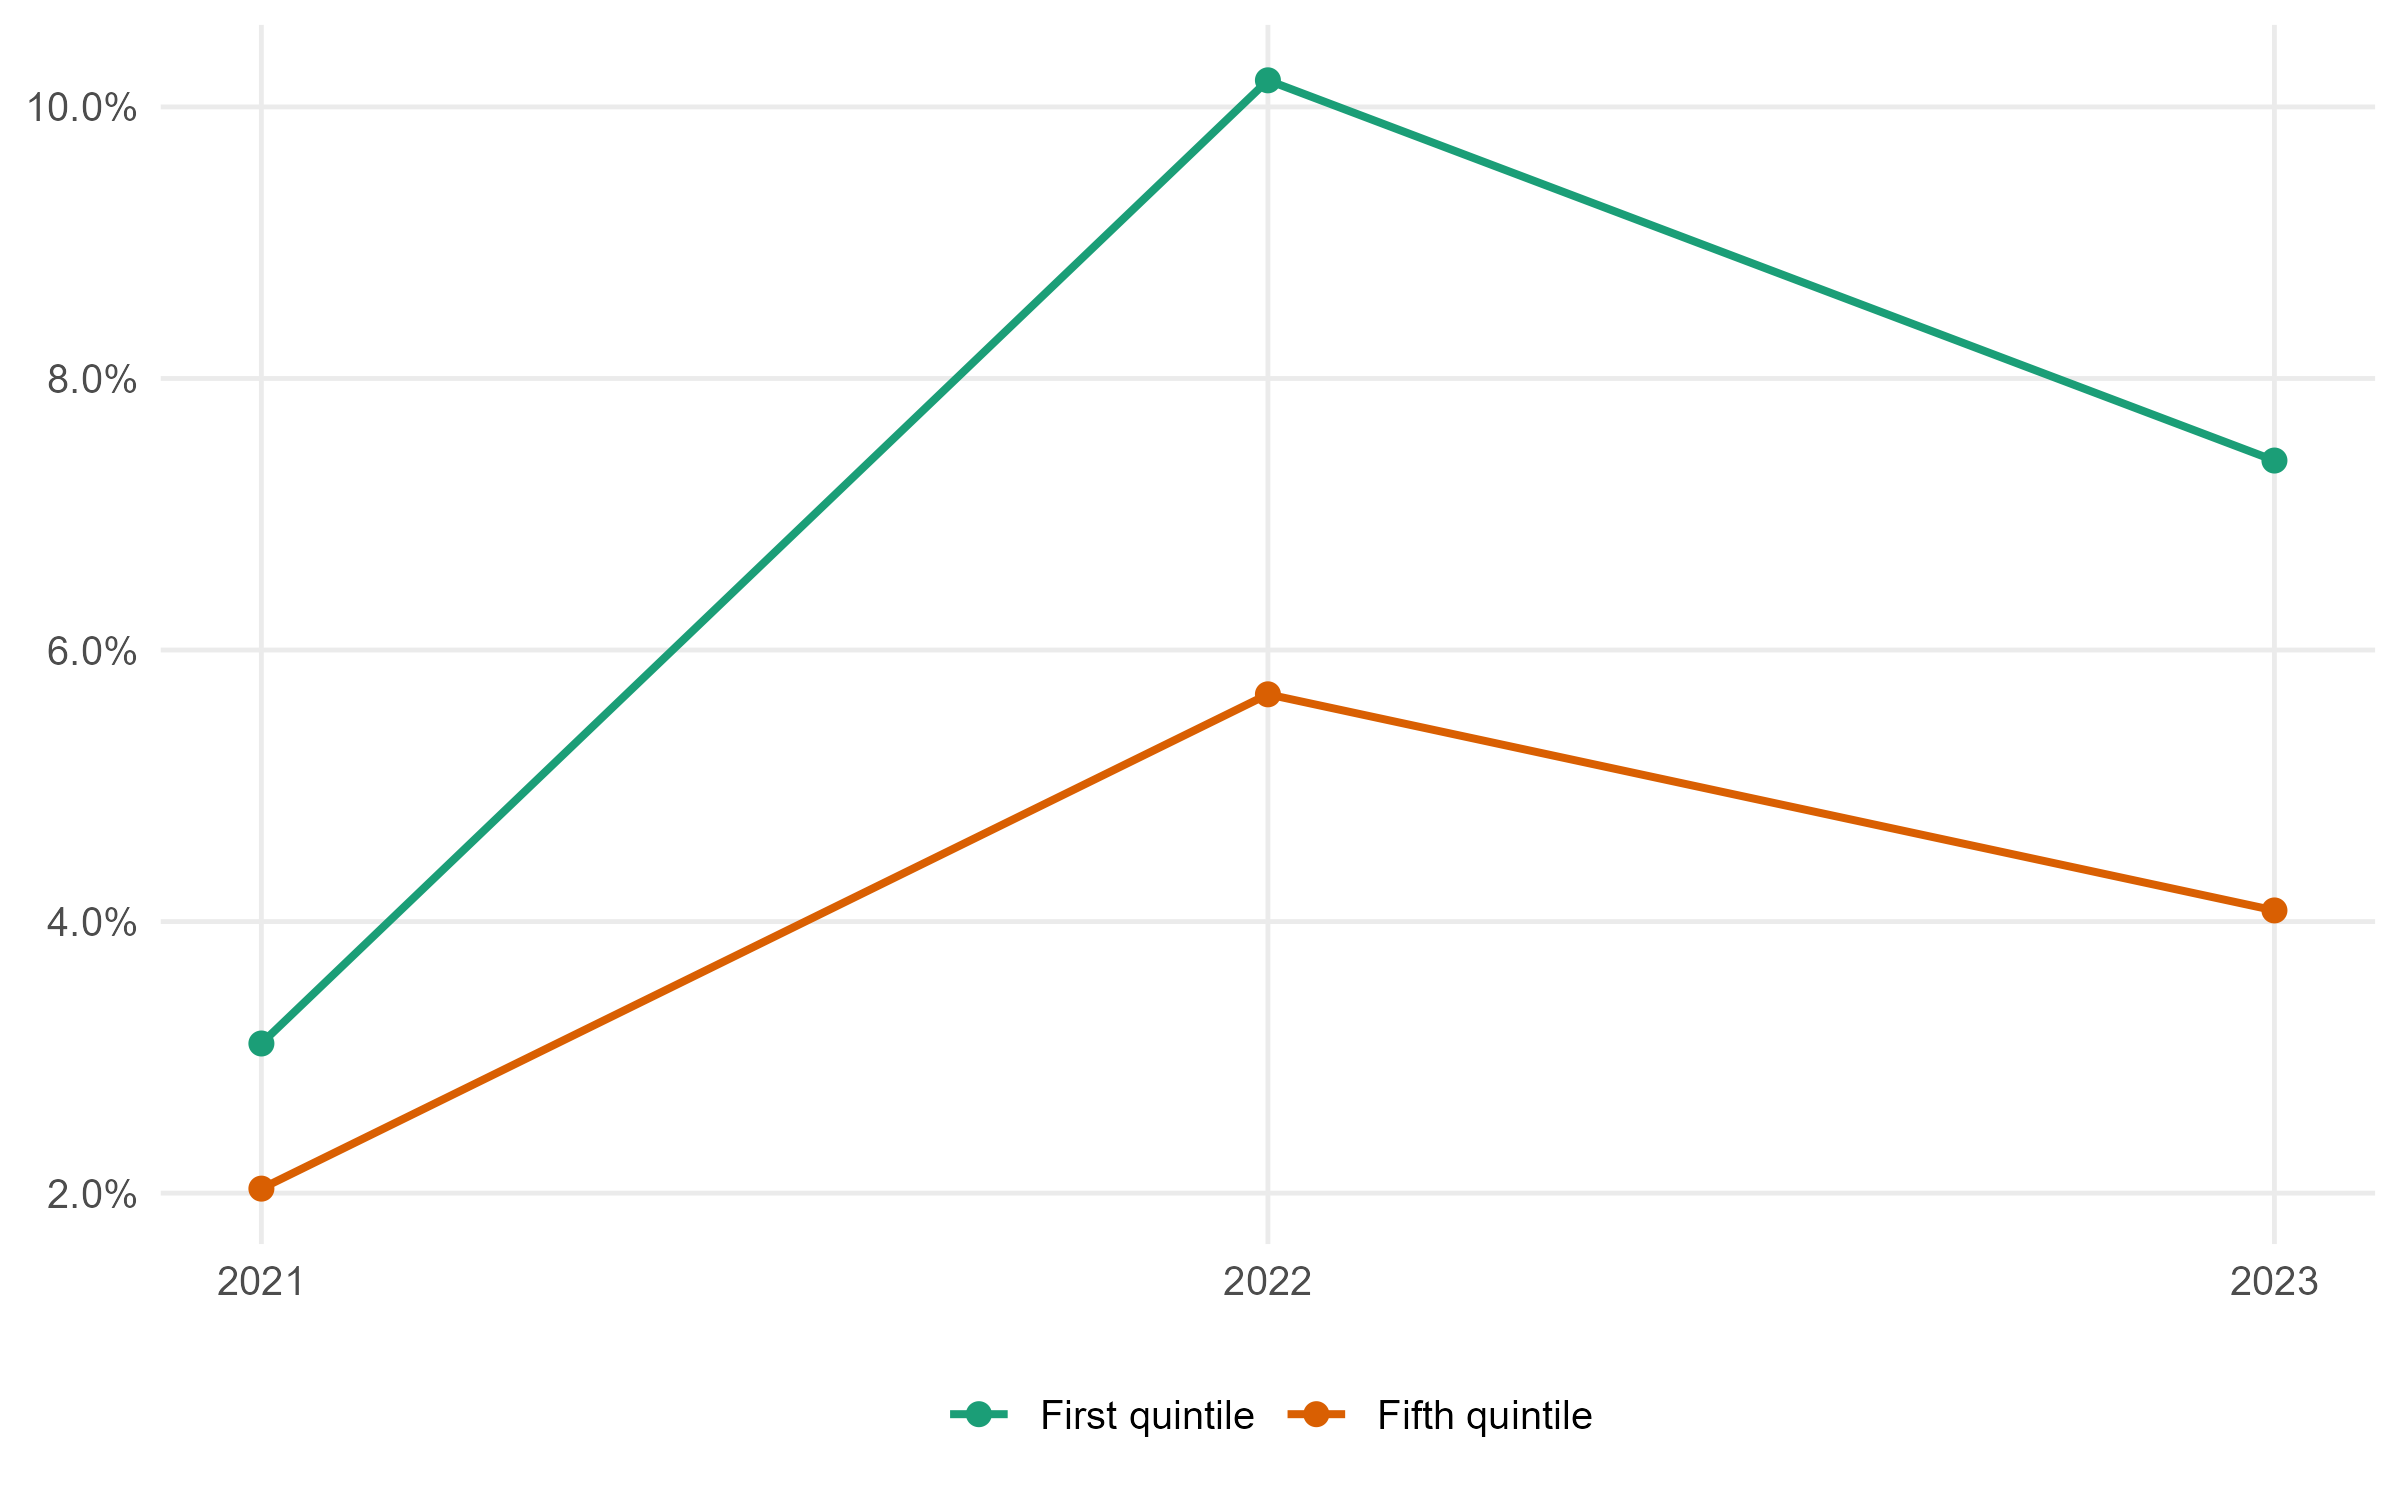
\includegraphics[width=0.70\textwidth,height=0.58\textheight,keepaspectratio]{fig/fig_EA20_2019_2026_income_inflation_burden_Q1_Q5.png}
\begin{itemize}
  \item The Q1 burden reached \textbf{3.1\%, 10.2\%, and 7.4\%} of net income in 2021--2023, versus \textbf{2.0\%, 5.7\%, and 4.1\%} for Q5.
\end{itemize}
\source{Eurostat HICP and HBS microdata; authors' calculations. Units: annual inflation burden, in percent of household net income.}
\end{frame}

% A4
\begin{frame}{The Paper Isolates the Household Expenditure Channel}
\begin{itemize}
  \item \textbf{Expenditure:} households buy different baskets, so relative-price shocks generate different inflation rates. This is the channel measured here.
  \item \textbf{Income:} wages, pensions, and transfers adjust at different speeds, producing unequal changes in real disposable income.
  \item \textbf{Wealth:} inflation erodes nominal assets and liabilities, transferring wealth from creditors to debtors.
  \item Our indices capture heterogeneity in expenditure shares within common COICOP price changes.
  \item They do not capture household-specific prices paid, product quality, within-category substitution, or the income and wealth channels.
\end{itemize}
\source{Main text; presentation framework adapted from the seminar PowerPoint.}
\end{frame}

% A6
\begin{frame}{Inflation Gaps Differ Sharply Across Countries}
\centering
\tiny
\renewcommand{\arraystretch}{0.78}
\setlength{\tabcolsep}{4pt}
\begin{tabular}{lrrrr}
\toprule
Country & Total inflation & Q1 inflation & Q5 inflation & Q1--Q5 gap\\
\midrule
Austria & 17.2 & 17.5 & 17.1 & 0.4\\
Belgium & 12.3 & 11.7 & 12.8 & -1.1\\
Croatia & 21.4 & 21.1 & 21.7 & -0.6\\
Cyprus & 12.0 & 12.7 & 12.0 & 0.7\\
Estonia & 33.0 & 38.7 & 31.2 & 7.5\\
Finland & 12.5 & 11.5 & 12.7 & -1.2\\
France & 12.2 & 12.3 & 12.1 & 0.2\\
Germany & 15.6 & 16.5 & 15.2 & 1.3\\
Greece & 14.7 & 15.1 & 14.5 & 0.6\\
Ireland & 14.9 & 17.2 & 13.3 & 3.8\\
Italy & 15.8 & 17.2 & 15.1 & 2.1\\
Latvia & 28.9 & 36.0 & 26.5 & 9.5\\
Lithuania & 30.4 & 33.6 & 29.0 & 4.6\\
Luxembourg & 11.4 & 11.0 & 11.1 & -0.2\\
Malta & 12.7 & 13.8 & 12.2 & 1.6\\
Netherlands & 16.9 & 17.7 & 16.5 & 1.2\\
Portugal & 14.2 & 13.1 & 15.4 & -2.3\\
Slovakia & 25.4 & 26.7 & 24.0 & 2.7\\
Slovenia & 18.1 & 19.9 & 17.5 & 2.4\\
Spain & 11.8 & 11.8 & 11.7 & 0.1\\
\midrule
\textbf{Euro area} & \textbf{14.7} & \textbf{15.2} & \textbf{14.4} & \textbf{0.9}\\
\bottomrule
\end{tabular}
\source{Eurostat HICP and HBS; authors' calculations. Units: cumulative inflation and Q1--Q5 gap, June 2021--June 2023, in percentage points.}
\end{frame}

% A7
\begin{frame}{Administered Prices Drive Most of the Gap Reduction}
\centering
\scriptsize
\setlength{\tabcolsep}{5pt}
\begin{tabular}{lrrr}
\toprule
Policy category & Fiscal cost & Average inflation & Q1--Q5 gap\\
 & (EUR bn) & effect (pp) & effect (pp)\\
\midrule
\multicolumn{4}{l}{\textit{Instrument classification}}\\
VAT cuts & 44.5 & -0.5 & -0.2\\
Administered prices & 161.0 & -1.1 & -0.9\\
Fuel subsidies and rebates & 25.4 & -0.2 & 0.1\\
Other calibrated layer & 37.1 & -0.2 & -0.2\\
\textbf{Total} & \textbf{268.0} & \textbf{-1.9} & \textbf{-1.1}\\
\midrule
\multicolumn{4}{l}{\textit{Targeted vs. untargeted}}\\
Untargeted price measures & 235.2 & -1.5 & -0.8\\
Targeted price measures & 32.8 & -0.4 & -0.4\\
\textbf{Total} & \textbf{268.0} & \textbf{-1.9} & \textbf{-1.1}\\
\bottomrule
\end{tabular}
\vspace{0.8em}
\begin{itemize}
  \item Negative values indicate that policies reduced inflation or the inflation gap.
\end{itemize}
\source{Bruegel; national sources for VAT food products; authors' calculations. Units: fiscal cost in EUR billions; average-inflation and Q1--Q5-gap effects, June 2021--June 2023, in percentage points.}
\end{frame}

\end{document}
